\documentclass[a4paper,fleqn,usenatbib]{mnras}

%=========================================================================
\usepackage{amsmath} 
\usepackage{amssymb} 
\usepackage{multirow}

\usepackage{graphicx}
\usepackage{grffile}
\usepackage[dvips]{epsfig}
\usepackage{epsfig}  
\usepackage{color}
\usepackage{caption}
\usepackage{hyperref}
\usepackage{bm}
%Non reposionated tables

%=========================================================================
%		INTERNAL MACROS
%=========================================================================
\def\be{\begin{equation}}
\def\ee{\end{equation}}
\def\ba{\begin{eqnarray}}
\def\ea{\end{eqnarray}}

% To highlight comments 
\definecolor{red}{rgb}{1,0.0,0.0}
\newcommand{\red}{\color{red}}
\definecolor{darkgreen}{rgb}{0.0,0.5,0.0}
\newcommand{\SRK}[1]{\textcolor{darkgreen}{\bf SRK: \textit{#1}}}
\newcommand{\SRKED}[1]{\textcolor{darkgreen}{\bf #1}}
\newcommand{\before}[1]{\textcolor{red}{ #1}}
\newcommand{\after}[1]{\textcolor{darkgreen}{ #1}}
\newcommand{\hs}{{\hspace{1mm}}}  
\newcommand{\tol}{Tololo 1214-277}
\newcommand{\rank}{\texttt{Ranked}}
\newcommand{\boot}{\texttt{Bootstrapped}}
\newcommand{\rand}{\texttt{Random}}
\newcommand{\HI}{{\text{H\MakeUppercase{\romannumeral 1}}} }
\newcommand{\HII}{{\text{H\MakeUppercase{\romannumeral 2}}} }
\newcommand{\lya}{\ifmmode{{\rm Ly}\alpha}\else Ly$\alpha$\ \fi}
\newcommand{\cm}{\ifmmode{{\rm cm}}\else cm\fi}
\newcommand{\ccm}{\,\mathrm{cm}^{-3}}
\newcommand{\ergps}{\,{\rm erg}\,{\rm s}\ifmmode{}^{-1}\else ${}^{-1}$\fi}
\newcommand{\Mpch}{\,{\rm Mpc}\,\ifmmode h^{-1}\else $h^{-1}$\fi}
\newcommand{\dd}{\mathrm{d}}
\newcommand{\vek}[1]{\bm{#1}}
\newcommand{\hb}{H$\beta$}
\newcommand{\ha}{H$\alpha$}
\newcommand{\oiii}{[OIII]}
\newcommand{\oii}{[OII]}
\newcommand{\nii}{[NII]}
\newcommand{\esca}{erg cm$^{-2}$ s$^{-1}$ \AA$^{-1}$}
\newcommand{\esc}{erg cm$^{-2}$ s$^{-1}$}
\newcommand{\es}{erg s$^{-1}$}
\newcommand{\esa}{erg s$^{-1}$}
\newcommand{\kms}{\ifmmode\mathrm{km\ s}^{-1}\else km s$^{-1}$\fi}
\newcommand{\hMsun}{{\ifmmode{h^{-1}{\rm{M_{\odot}}}}\else{$h^{-1}{\rm{M_{\odot}}}$}\fi}}
\newcommand{\Msun}{{\ifmmode{{\rm{M_{\odot}}}}\else{${\rm{M_{\odot}}}$}\fi}}

\newcommand{\jefr}[1]{\textcolor{darkgreen}{\bf JEFR: \textit{#1}}}

\begin{document}

%=========================================================================
%		FRONT MATTER
%=========================================================================
\title[LG satellites distribution asphericity]{We are not the 99 percent: quantifying
  asphericity in the distribution of Local Group satellites}
\author[J.E. Forero-Romero \& V. Arias]
{Jaime E. Forero-Romero $^{1}$ \thanks{je.forero@uniandes.edu.co},
Ver\'onica Arias$^1$\\
%%
$^1$ Departamento de F\'isica, Universidad de los Andes, Cra. 1
  No. 18A-10 Edificio Ip, CP 111711, Bogot\'a, Colombia \\
}

\maketitle

\begin{abstract}
We use numerical simulations to build an explicit probability
distribution for the asphericity in the satellite distribution around
galaxies similar to the Local Group (LG) in the Lambda Cold Dark
Matter (LCDM) paradigm. 
This allows us to estimate the atipicallity
of the satellite distributions in the LG even when the underlying
simulations do not have enough systems that fully resemble the LG.
We demonstrate the method using three different simulations:
Illustris-1,  Illustris-1-Dark and ELVIS. 
Detailed results differ among the simulations suggesting a strong
influence of the typical Dark Matter (DM) halo mass in the LG samples.
However, there are three common trends.
First, at most of $2\%$ the pairs are expected to have satellite
distributions with the same asphericity as the LG; second,
between $27\%$ to $56\%$ of the pairs have a halo with a satellite
distribution as aspherical as in M31; and third, at most $3\%$ of the
pairs have a satellite distribution as planar as in the MW. 
The brightest satellites in the M31 galaxy have a rather typical
distribution in the LCDM context, while the MW distribution is
atypical in this respect.  
These quantitative results place the LG at the level of a $3\sigma$
outlier in the LCDM paradigm. 
We suggest that to understand this atipicality will require quantifying
the probability distribution for the satellite distribuition
asphericity as a function of halo mass and large scale environment. 
The approach presented here can facilitate that study and other comparisons
between different numerical setups and choices to study satellites
around LG pairs in simulations.  
\end{abstract}

\begin{keywords}Galaxies: halos --- Galaxies: statistics --- Dark
  Matter --- Methods: numerical  
\end{keywords}

\section{Introduction}

The spatial distribution of satellite galaxies around our Milky Way
(MW) and the M31 galaxy is becoming a stringent test for structure
formation theories in a explicit cosmological context. 

This started with the suggestion of a Magellanic Plane, a flattened
structure of satellite galaxies and globular clusters around the MW,
first suggested by \cite{1976RGOB..182..241K} and \cite{1976MNRAS.174..695L}.  
\cite{2005A&A...431..517K} then quantified that the
highly planar distribution of the 11 classical MW satellites has less
than a $0.5\%$ chance  to happen by chance if the
parent distribution is spherically symmetric, interpreting this as a
challenge to the Lambda Cold Dark Matter (LCDM) paradigm.
The same year it was recognized, using numerical simulations, that
this comparison was unfair given that Dark Matter halos in LCDM
are expected to be triaxial and not spherical
Nevertheless, some estimates of the chances to find simulated satellites as
planar as in the MW 
were as low as $2\%$ \citep{2005ApJ...629..219Z} while others expected
planar satellite configurations in every DM halo
\citep{2005MNRAS.363..146L}.




Later, \cite{2007MNRAS.374.1125M} used simulations to confirm the low
chances ($<0.5\%$) found in \cite{2005A&A...431..517K}.
This result was challenged by \cite{2009MNRAS.399..550L} who continued
to report high chances to find a planar configuration;
two more recent numerical experiment with high resolution simulations
(\cite{2013MNRAS.429..725S} and \cite{2016MNRAS.457.1931S}) reported
contradicting results (low and high chances to find the observational
result, respectively) but precise figures are not quoted in either of
these three reports. 
Meanwhile, \cite{2013MNRAS.429.1502W} and \cite{2014ApJ...789L..24P} published
the results new tests using high resolution simulations and cosmological
volumes arriving at a chance of $6\%$ and $0.77\%$, respectively, to
have a satellite distribution as triaxial as the observations. 


In the case of M31, observational studies have found a planar satellite
distribution in a special subset of $15$ satellites out of the 
total poulation of $27$ satellites \citep{2013ApJ...766..120C,
2013Natur.493...62I}, although considering the satellites ranked by
luminosity does not show any special feature.
All published studies agree on the point that the spatial distribution of
the 15 to 27 brightest satellites are consistent with  spherically
symmetric distribution and easy to reproduce in LCDM simulations
\citep{2006AJ....131.1405K,2007MNRAS.374.1125M, 2013ApJ...766..120C}.    
Table \ref{table:M31} and Table \ref{table:MW} summarize some more
details on the results we have just mentioned \footnote{
Those tables also include the results from this paper using the
methodolgy we describe in the upcoming sections.}.


\begin{table*}
\centering
\begin{tabular}{|p{4.0cm}|p{4.5cm}| p{5.5cm}| c|}\hline
Reference & Target Measurement & Parent Simulation & Probability ($\%$)\\\hline
\text{\cite{2006AJ....131.1405K}} & RMS height in 15 brightest
satellites & Monte Carlo satellite distributions with a power law
radial distribution & $87-99$\\
\text{\cite{2007MNRAS.374.1125M}} & Triaxiality and RMS height in 16 brightest satellites & Monte Carlo from an spherical power law radial
distribution & $17$\\
\text{\cite{2013ApJ...766..120C}}& RMS height in the 27 brightest
satellites & Monte Carlo randomized satellite distribution & High\\
This Work & Triaxiality and RMS height in 11-15 brightest
satellites & 24 halos from selected pairs in a cosmological N-body Dark Matter only simulation ($\sim
10^{6}$\Msun particle mass resolution)& 56 \\
This Work & Triaxiality and RMS height in 11-15 brightest
satellites & 20 halos from selected pairs in a cosmological N-body hydro simulation ($\sim
10^{6}$\Msun particle mass resolution)& 27 \\
This Work & Triaxiality and RMS height in 11-15 brightest
satellites & 12 high resolution DM only N-body simulations ($\sim
10^{5}$\Msun particle mass resolution) of halo pairs & 37 \\
\hline
\end{tabular}
\caption{Probability to find  the triaxiality and/or root mean squared
  (RMS) height of M31 satellites in LCDM simulations. 
\label{table:M31}}
\end{table*}


\begin{table*}
\centering
\begin{tabular}{|p{4.0cm}|p{4.5cm}| p{5.5cm}| c|}\hline
Reference & Target Measurement & Parent Simulation & Probability ($\%$)\\\hline
\text{\cite{2005A&A...431..517K}} & RMS height in 11 classical
satellites & Monte Carlo from an spherical power law
radial distribution. & $<0.5$ \\
\text{\cite{2005MNRAS.363..146L}} & Triaxiality of 11 classical
satellites & 6 high resolution DM only N-body simulations ($\sim10^5$
\Msun\ particle mass resolution). & High\\ 
\text{\cite{2005ApJ...629..219Z}} & Triaxiality and disk height in 
11 classical satellites & 3 high resolution DM only N-body
simulations. ($\sim10^6$ \Msun\ particle mass resolution) & 2 \\
\text{\cite{2007MNRAS.374.1125M}} & Triaxiality and RMS height in 11-13 brightest satellites & Monte Carlo from a halo triaxiality distribution from LCDM
simulations & $<0.5$\\
\text{\cite{2009MNRAS.399..550L}}& Triaxiality in 11 classical satellites & 436 halos from a
cosmological N-body simulation ($1.3\times 10^{8}$\Msun\ particle mass)
&  High \\
\text{\cite{2013MNRAS.429..725S}}& $c/a$ ratio in 12 brightest
satellites & 6 High resolution DM only N-body simulations ($\sim
10^3$\Msun particle mass resolution) of individual halos & Low \\
\text{\cite{2013MNRAS.429.1502W}}& $c/a$ ratio or RMS height in 11 brightest
satellites & 1686 halos from a cosmological DM only N-body simulation
($\sim 10^6$\Msun particle mass resolution) & 6 or 13 \\
\text{\cite{2014ApJ...789L..24P}}& $c/a$ and $b/a$ ratio in 11
classical satellites & 48 high resoltion DM only N-body simulations
($\sim 10^{5}$\Msun particle mass resolution) of both halo pairs and
isolated halos & 0.77\\
\text{\cite{2016MNRAS.457.1931S}}& $c/a$ ratio in 11 classical satellites & 12
high resolution Hydro simulation of halo pairs ($\sim 10^{4}$\Msun particle
mass resolution) & High\\
This Work & Triaxiality and RMS height in 11-15 brightest
satellites & 24 halos from selected pairs in a cosmological N-body
Dark Matter only simulation ($\sim 10^{6}$\Msun particle mass resolution)& 3\\
This Work & Triaxiality and RMS height in 11-15 brightest
satellites & 20 halos from selected pairs in acosmological N-body
hydro simulation ($\sim 10^{6}$\Msun particle mass resolution)& 0.6 \\
This Work & Triaxiality and RMS height in 11-15 brightest
satellites & 12 high resolution DM only N-body simulations ($\sim
10^{5}$\Msun particle mass resolution) of halo pairs & 0.2 \\
\hline
\end{tabular}
\caption{Same as Table \ref{table:M31} for the MW satellites.
\label{table:MW}}
\end{table*}


Some of the difficulty in trying to reconcile and understand the
seemly conflicting or inconclusive results on the MW has its origin on
the frequentist fashion generally used to compute probabilities.
Usually, this process starts by building a high level parent sample in the
simulation and then counting how many elements has a subset
meeting some criteria. This has two incovenients.
The first is that the probability estimate is made against whatever
turns out to be typical in each simulation. 
A fair comparison across simulations would require first
characterizing all the simulations at the high level parent samples,
something that is difficult to do in practice. 
The second inconvenient is that the systems that fully resemble
the LG (i.e. its stellar mass content, morphology or kinematics) have
a low cosmological number density, this means that for the current
cosmological volumes in simulations the high level parent sample has a
small size, making it hard to derive robust probabilities by counting.   


In this paper we control the first effect by setting as a direct 
point of reference an spherical satellite distribution and not the
simulations themselves.
The spherical satellite distribution is built from the data itself
(observational or simulated) by randomizing the angular position
of each satellite around the central galaxy and keeping its radial
distance fixed \citep{2017AN....338..854P}. 
We characterize the satellites in terms of the scalars describing its
deviation from the spherical distribution. 
We then build an explicit analytic
probability distribution for the deviations from asphericity; this
solves the problem of having a common reference point to compare
simulations. 
We then use different simulations to estimate the parameters in this
distribution to later use it as a parent sample to generate any
desired number of samples that are by construction statistically
compatible with simulations; thus overcoming the problem of having a small
number of systems in the parent simulations.

To summarize, we use asphericity to characterize in the
on equal footing simulations and observations. 
Then, we build an explicit probability distribution for the asphericity and
use simulations to estimate the parameters in this distribution. 
Finally, we use these distributions to generate large number of
samples and directly estimate the number of systems meeting a desired
set of criteria.

The rest of the paper describes in detail our implementation and
results. It is structured as follows. 
In Section \ref{sec:DataSamples} we list the sources of the observational and
simulated data to be used throughout the paper.
In Section \ref{sec:SpatialMeasurements} we describe the methods we
use to build halo pairs and  
characterize its satellite distributions.
In Section \ref{sec:results} we present our results to finally
conclude in Section \ref{sec:conclusions}. 



\section{Data samples}\label{sec:DataSamples}

\subsection{Observational Data}
\label{sec:obs}

The base for our analysis is the catalog compiled in
\citep{2014yCat..74351928P} which reports information on all 
galaxies within 3 Mpc around the Sun to that date. 
Detailed description of the compiled catalog can be found in
\citep{2013MNRAS.435.1928P}, here we summarize the relevant features
for the current study.

The information in the catalogue is based on the catalogue compiled by
\cite{2012AJ....144....4M}.
The distance estimates are based on resolved stellar populations. 
We use three dimensional positions in a cartesian coordinate system
as computed by \cite{2013MNRAS.435.1928P}.
In this coordinate system the $z$-axis points towards the Galactic north pole, the
$x$-axis points in the direction from the Sun to the Galactic centre,
and the $y$-axis points in the direction of the Galactic rotation.


For both the M31 and MW we only use the 11 to 15 brightest satellites (using
$M_V$ magnitudes) within a distance of $300$kpc to its central galaxy.
The satellites included for the MW analysis are: 
LMC, SMC, Canis Major, Sagittarius dSph, Fornax, Leo I, Sculptor,
Leo II, Sextans I, Carina, Ursa Minor, Draco, Canes Venatici (I),
Hercules and Bootes II.
The satellites included for the M31 analysis are: Triangulum, NGC205,
M32, IC10, NGC185, NGC147, Andromeda VII, Andromeda II, Andromeda
XXXII, Andromeda XXXI, Andromeda I, Andromeda VI, Andromeda XXIII, LGS 3, 
 and Andromeda III.



\subsection{Data from the Illustris project}
\label{sec:illustris}

We use publicly available data from the Illustris Project 
\citep{2014MNRAS.444.1518V}. 
This suite of cosmological simulations, performed using the quasi-Lagrangian
code AREPO \citep{2010MNRAS.401..791S}, followed the coupled evolution of dark 
matter and gas and includes parametrizations to account for the effects of
gas cooling, photoionization, star formation, stellar feedback, black
hole and super massive black hole feedback. 
The simulation volume is a cubic box of $75$ \Mpch\ on a side.
The cosmological parameters correspond to a $\Lambda$CDM cosmology
consistent with WMAP-9 measurements \citep{2013ApJS..208...19H}. 

We extract halo and galaxy information from the Illustris-1 and
Illustris-1-Dark simulations, the former simulation includes
hydrodynamics and star formation prescriptions while the latter only
includes dark matter physics.
These simulations have the highest resolution in the current release of the
Illustris Project.
Illustris-1 has $1820^3$ dark matter particles and $1820^3$ initial gas
volumen elements, while Illustris-1-Dark has $1820^3$ dark matter particles.
This corresponds to a dark matter particle mass of
$6.3\times 10^6$\Msun\ and a minimum mass for the baryonic volume
element of $8.0\times 10^7$\Msun for Illustris-1 and a dark matter
particle mass of $7.6\times 10^6$\Msun for Illustris-1-Dark.
In both simulations the dark matter gravitational softening is $1.4$
kpc.

We buid a sample of pairs that resemble the conditions in the LG.
To construct this sample we select from Illustris-1 all galaxies with a stellar
mass in the range $1\times10^{10}\Msun <M_{\star}<1.5 \times 10^{11}
\Msun$.
Then we select the pairs with the following conditions.

\begin{itemize}
\item For each galaxy $A$ we find its closest galaxy $B$, if galaxy $A$ is also
the closest to halo $B$, the two are considered as a pair. 
\item With $d_{AB}$ the distance between the two galaxies and
  $M_{\star,min}$ the lowest stellar mass in the two galaxies, we
  discard pairs that have any other galaxy $C$ with stellar mass
  $M_{\star}>M_{\star, min}$ closer than $3\times d_{AB}$ from any of
  the pair's members. 
\item The distance $d_{AB}$ is greater than $700$ kpc.
\item The relative radial velocity between the two galaxies, including
  the Hubble flow, is $-120\ \kms <v_{AB,r}<0\ \kms$. 
\end{itemize}

We find 27 pairs with these conditions. 
We then select the pairs where in both halos there are at least 15
detected subhalos, thus discarding pairs with halos with the lowest
mass.
We end up with a total of 20 pairs in Illustris-1.
In Illustris-1-DM we use the center of mass position of the 27 pairs
in Illustris-1 to find the matching halo pairs.
After discarding the pairs with less than 15 detected subhalos in one
of the halos we end up with a total of 24 pairs. 
This corresponds to a pair number density of $\sim 2 \times10^{-5}$
pairs Mpc$^{-3}$ 
Appendix A shows the physical  properties (stellar masses, maximum
circular velocities, radial velocities and separation) of those
pairs.

Although Illustris-1 has stellar particles, we do not use their
properties to select the satelite population because the smallest
galaxies are barely resolved in stellar mass at magnitudes of
$M_V=-9$, close to the limit of the 11 ``classical'' MW satellites.
We use instead the dark matter information as the smallest sub-halos
we care about are sampled with at least $40$ particles.  
%comentario: este último criterio no me parece que esté claramente
%descrito

Both in Illustris-1 and Illustris-1-DM we chose the satellite samples
by ranking the subhalos in decreasing order of its current maximum
circular velocity and select the first $N_p$ halos in the list.  
The results presented here correspond to $11\leq N_p\leq 15$. 

\subsection{Data from the ELVIS project}
\label{sim:ELVIS}

We use data from the public release of the Exploring the Local
Universe In Simulations (ELVIS) project.
For a detailed description of that project and its data we refer the
reader to \cite{2014MNRAS.438.2578G}. 
Here we summarize the elements relevant to our discussion.

ELVIS data comes from resimulations of dark matter halo pairs selected
in dark matter only cosmological simulations. 
The parent cosmological boxes have a cosmology consistent with the
Wilkinson Microwave Anisotropy Probe 7 results.


The ELVIS project used the results from $50$ simulation boxes of side
lenght $70.4$ Mpc to select pairs with kinematic characteristics
similar to the LG. 
These selection criteria included the following
\begin{itemize}
\item The virial mass of each host must be in the range 
$1\times
  10^{12} M_{\odot}< M_{vir}<3\times 10^{12}M_{\odot}$ 
\item The total pair mass must be in the range
$2\times
  10^{12} M_{\odot}< M_{vir}<5\times 10^{12}M_{\odot}$ 
\item The center of mass separation is in the range $0.6\leq d\leq1$
  Mpc.
\item The relative radial velocity is negative.
\item No halos more massive than the least massive halo within $2.8$
  Mpc and no halos with $M_{vir}>7\times 10^{13}$ within $7$ Mpc of
  the pairs' center of mass.
\end{itemize} 

This corresponds to a pair number density of $\sim 8 \times10^{-6}$ pairs
Mpc$^{-3}$, this is a factor $\sim 2.5$ lower than the pair number density
we find in the Illustris data.
There were a total of 146 pairs that met those criteria, but only $12$
were chosen for resimulation. 
Additionally, the selected pairs for resimulation have a relative
tangential velocity less than $75 $\kms. 
The dark matter particle resolution in these resimulations is
$1.9\times 10^5$, a thousand times larger than Illustris-1.
In this paper we only use the results from these $12$ resimulated pairs.

Appendix A compares the physical properties (stellar masses, maximum
circular velocities, radial velocities and separation) in those
pairs against the results from the Illustris-1 simulations.

\section{Building, Characterizing and Comparing Satellites Spatial Distributions}
\label{sec:SpatialMeasurements}


\subsection{Building Satellite Samples}

We compare the joint satellite distributions in the MW and M31 at fixed
satellite number, $N_s$.
This means that the magnitude cut corresponding to the faintest
satellite included in the sample is different in each case.
We make this choice for two reasons. 
First, to be sure that there is a non-zero number of satellites in the
simulations to make the computations.  
Second, to rule out the influence of satellite numbers in the
statistics. 

We compute the satellite statistics for 11 up to 15 satellites.
The lower limit corresponds to the number of classical Milky Way
satellites.
The upper limit corresponds to the maximum number of satellites that
can be resolved in both halos for most of the isolated pairs in Illustris-1.
In simulations we rank the subhalos by their maximum
circular velocity, in observations we rank the satellites by its $M_V$
magnitude. 

We also use two kinds of satellite distributions. 
The first keeps the positions for the satellites fixed as provided in
the observations/simulations; the second randomizes the angular positions of
the satellites around the central galaxy while keeping its radial
distance fixed. The randomization process is done 1000 times for each
galaxy. 



\begin{table*}
  \centering
  \renewcommand{\arraystretch}{1.2}
  \begin{tabular}{|p{2.5cm}|c|c|c|c|c|c|}
    \hline
    \multirow{2}{4.0cm}{} & \multicolumn{2}{c|}{\textbf{Observations}}
    & \multicolumn{2}{c|}{\textbf{Randomized Obs.}} &
    \multicolumn{2}{c|}{\textbf{Normalized Units}}\\
    % \hline
    % \textbf{Inactive Modes} & \textbf{Description}\\
    \cline{2-7}
    & \textbf{M31} & \textbf{MW} & \textbf{M31} & \textbf{MW} & \textbf{M31} & \textbf{MW} \\
    %\hhline{~--}
    \hline
    Plane width (kpc) & $59\pm 3$  & $21\pm 2$  & $65\pm 12$   &
    $45\pm 8$    & $-0.48\pm 0.24$ & $-2.48\pm 0.26$\\\hline
    $c/a$ ratio & $0.45\pm 0.04$ & $0.25\pm 0.05$ & $0.55\pm0.10$ &
    $0.53\pm 0.10$ & $-1.03\pm 0.37$ & $-2.18\pm 0.42$\\ \hline
    $b/a$ ratio & $0.82\pm 0.06$ & $0.80\pm 0.04$ & $0.82\pm0.07$ &
    $0.81\pm 0.08$ & $-0.02\pm 0.82$ & $-0.13\pm 0.47$\\ \hline
  \end{tabular}
  \caption{Results from observations. Mean values and standard deviations for the different
    quantities describing the satellite distributions: plane width, $c/a$
    ratio and $b/a$ ratio. 
    The first colum refers to the results from
    observational data, the second column uses the spherically
    randomized version of the observational data, the third column
    corresponds to the observational data recentered and normalized
    by the randomized values. \label{table:observations}}
\end{table*}


\begin{table*}
  \centering
  \renewcommand{\arraystretch}{1.2}
  \begin{tabular}{|p{2.5cm}|c|c|c|c|c|c|}
    \hline
    \multirow{2}{4.0cm}{} & \multicolumn{2}{c|}{\textbf{Illustris-1-Dark}} & \multicolumn{2}{c|}{\textbf{Illustris-1}} & \multicolumn{2}{c|}{\textbf{ELVIS}}\\
    % \hline
    % \textbf{Inactive Modes} & \textbf{Description}\\
    \cline{2-7}
    & \textbf{M31} & \textbf{MW} & \textbf{M31} & \textbf{MW}& \textbf{M31} & \textbf{MW}\\
    %\hhline{~--}
    \hline
    Plane width (kpc) & $62\pm 3$   & $61\pm 3$     & $70\pm 4$ & $67\pm 2$ & $70\pm 2$& $68\pm 4$ \\\hline
    $c/a$ ratio & $0.50\pm0.01$ & $0.50\pm 0.02$ & $0.52\pm 0.01$ & $0.53\pm 0.01$ & $0.54\pm 0.01$& $0.49\pm 0.02$ \\ \hline
    $b/a$ ratio & $0.79\pm0.01$ & $0.81\pm 0.02$ & $0.80\pm 0.01$ & $0.80\pm 0.02$ & $0.80\pm0.01$& $0.81\pm 0.01$\\ \hline
  \end{tabular}
  \caption{Results from simulations. Mean values and standard deviations for the different
    quantities describing the satellite distributions: plane width, $c/a$
    ratio and $b/a$ ratio. 
    The first column summarize the results from the 24 pairs in
    Illustris-1-Dark, the second column from the 20 pairs in
    Illustris-1 and the third column from the 12 pairs in the
    ELVIS project.\label{table:simulations}}
\end{table*}



\subsection{Describing Samples with the Inertia Tensor}
We base describe the satellites with the inertia
tensor defined by the satellites' positions.  

\begin{equation}
{\bf{\bar{I}}} = \sum_{k=1}^{N_s}[(\bf{r}_i - \bf{r}_0)^2\cdot \bf{1} -
  (\bf{r}_i-\bf{r}_0)\cdot (\bf{r}_i - \bf{r}_0)^{T}],
\label{eq:intensor}
\end{equation}
%
where $k$ indexes the set of satellites of interest
$\bf{r}_k$ are the satellites' positions, $\bf{r}_{0}$ is the location
of the central galaxy $\bf{1}$ is the unit matrix, and  
${\bf r}^T$ is the transposed vector $\bf{r}$. 
We use $\bf{r}_0$ as the position of the central galaxy, and not the
satellites' geometrical center, to allow for a fair comparison once
the angular positions of the satellites are randomized around this
point. 

From this tensor we compute its eigenvalues,
$\lambda_1>\lambda_2>\lambda_3$, and corresponding eigenvectors,
$\hat{I}_1$, $\hat{I}_2$, $\hat{I}_3$.
We define the size of the three ellipsoidal axis as
$a=\lambda_1$, $b=\lambda_2$ and $c=\lambda_3$.
We also define $\hat{n}\equiv \hat{I}_1$ as the vector perpendicular to the
planar satellite distribution. 
We also define the Root Mean Squared (RMS) width $w$, of the planar
satellite distribution, as the standard deviation of the satellite
distances to the plane defined by the vector $\hat{n}$.   

To summarize we characterize the satellite distribution by for
quantities obtained from the inertia tensor: 
\begin{itemize}
\item RMS plane width, $w$.
\item $c/a$ axis ratio.
\item $b/a$ axis ratio.
\end{itemize}


\subsection{Comparing Satellite Samples}

We compare each satellite distribution against its own spherically
randomized distribution.
We keep fixed the radial position of every satellite
with respect to the central galaxy and then randomize its angular
position. 
We repeat this procedure 1000 times for each satellite distribution
and proceed to measure the quantities mentioned in the previous section:
$w$, $c/a$ and $b/a$.
For each quantity we compute the average and standard deviation from
the 1000 random samples. 
This allows us to build a normalized version of all quantities of
interest by substracting the mean and dividing between the standard
deviation of the randomized samples.

This allows us to make a first comparison. 
The observed/simulated
distribution against its randomized version. 
The second intermediate comparison we make is of the observations against
the simulations.
The final comparison is between the normalized quantities, both
observed and simulated.

The comparison between the normalized quantities is the one that
carries the important information about the deviations from
spheriticy. 
We do not want to directly compare how the observations
deviate from simulations but to compare the deviations from
asphericity in observations and simulations. 


\subsection{Describing joint satellite distributions}

After building the normalized variables with the simulated data we
perform a Kolmogorov-Smirnov test with the null hypothesis of belonging
to a normal distribution with mean and standard deviation computed
from the mean and standard deviation from the data itself. 
We find that the distributions for the normalized $w$, $c/a$ and $b/a$
are consistent with gaussian ditributions.


Based on this result we build a multivariate normal distribution for
the joint distributions of the normalized $w$, $c/a$ and $b/a$:

\begin{equation}
p(X; \mu, \Sigma) = \frac{1}{(2\pi)^{3/2}|\Sigma|^{1/2}}
\exp\left(-\frac{1}{2}(X-\mu)^{T}\Sigma^{-1}(X-\mu)\right), 
\label{eq:multivariate}
\end{equation}
% 
where $X=[w, c/a, b/a]^{T}$ is a vector variable with the normalized
quantities, $\mu$ is the vector mean and the $\Sigma$ is the
covariance matrix.  

We compute the preferred covariance matrix and the mean distribution values
with a jackknife technique. 
That is, out of the the $n$ pairs we have, we perfom $n$ different
covariance and mean value measurements using only $n-1$ pairs. 
The reported covariance and mean values correspond to the average of
all measurements, the corresponding standard deviation also helps us to
estimate the uncertainty on every reported coefficient.
This compact description allows us to generate samples of size $N$
that are consistent by construction with their parent simulation. 

Finally, we use the generated samples to estimate how
common are the deviations from sphericity that we measure in the
observational data.  
We use a double-tailed test in this comparison, meaning that we
always measure the fraction of points with absolute values larger than the
treshold absolute observed value. 


% referencia posiciones satellites
% http://adsabs.harvard.edu/abs/2013MNRAS.435.1928P

\begin{figure*}
\centering
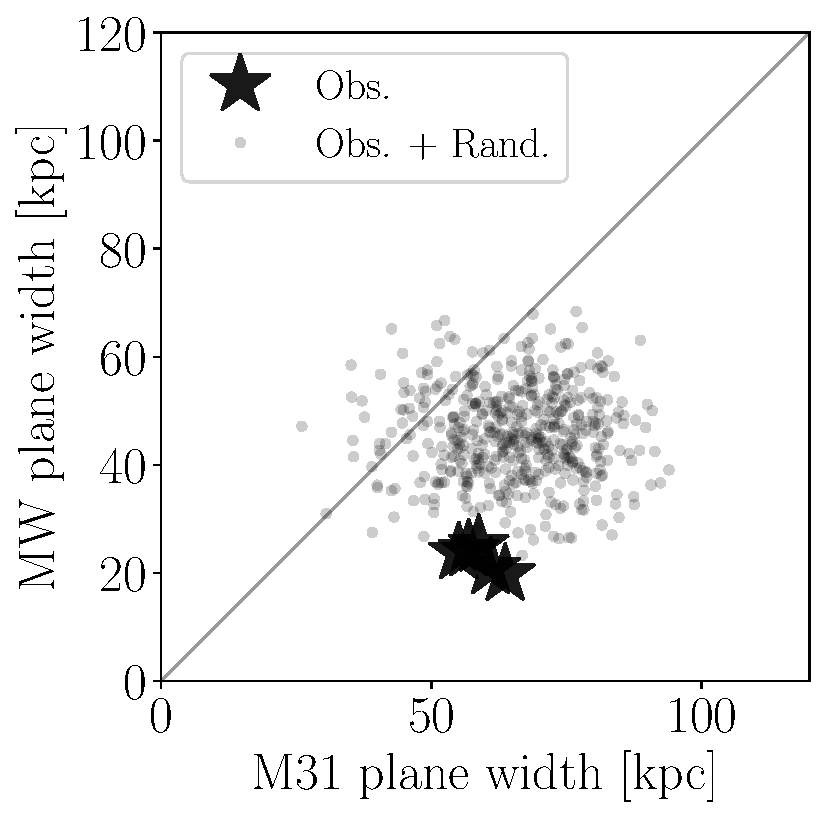
\includegraphics[width=0.30\textwidth]{scatter_random_ranked_width.pdf}
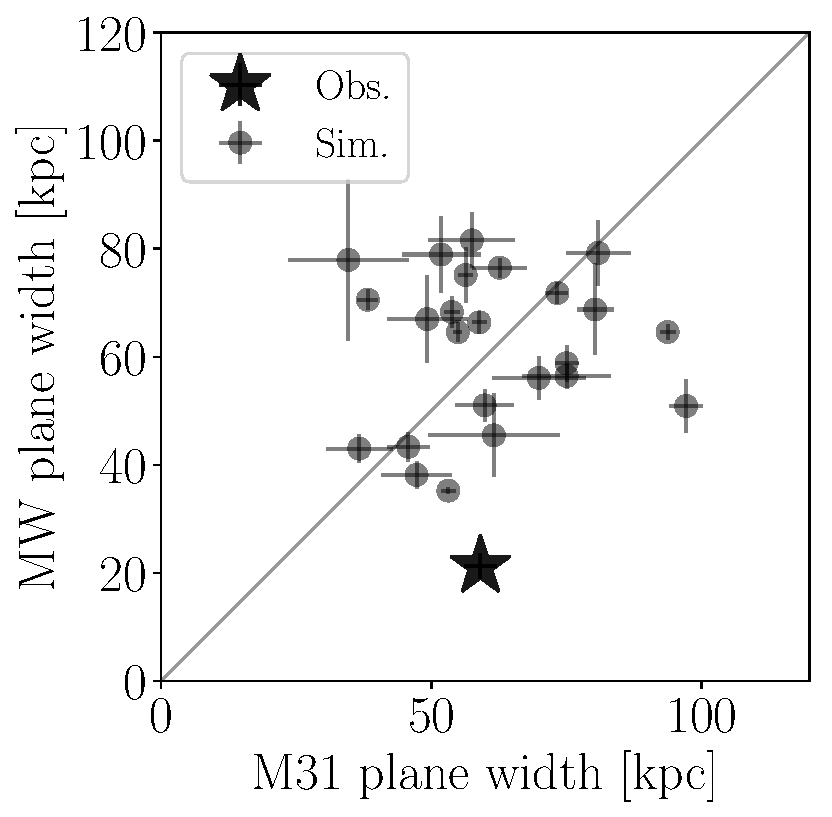
\includegraphics[width=0.30\textwidth]{scatter_ranked_illudm_width.pdf}
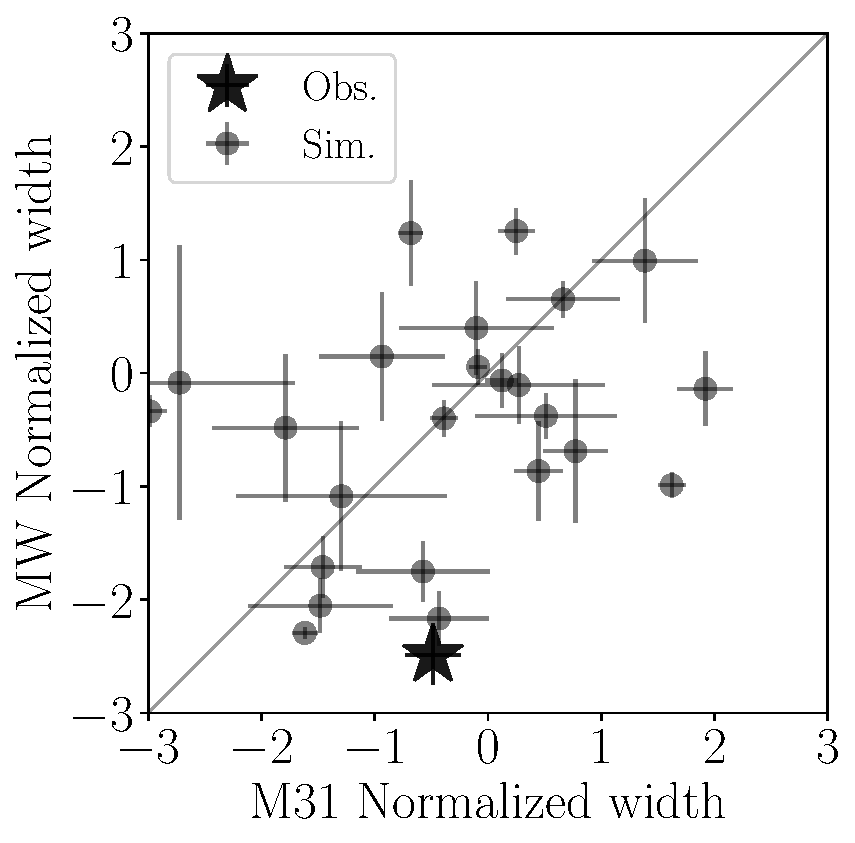
\includegraphics[width=0.30\textwidth]{scatter_norm_ranked_illudm_width.pdf}
\caption{Plane width characterization in observations and
  simulations (Illustris1-Dark in this case). In all panels the
  horizontal/vertical axis corresponds to the  M31/MW or the
  most/less massive halo in the pair 
  Left. Plane width in physical units comparing the results from observations
(stars) against the result of spherically randomizing the satellite
positions (circles). 
Middle. Average from the observations (star) and the average from each
pair in the simulation (circles).
Right. Same as the middle panel except that this time each point has
been normalized (median substracted and normalized by the standard
deviation) to the results of its randomization. 
The main message of these panels is that the MW has a significantly
thinner plane both compared to the result of its own satellite
spherical randomization (left panel) and the expectation from
simulations (middle and right panel).  
This low value is $2\sigma$ away from what is expected in a spherical
distribution. 
In M31 the satellite distribution is in agreement with the
expectations both from an spherical distribution and the results form the
simulations. 
\label{fig:scatter_width}}
\end{figure*}


\begin{figure*}
\centering
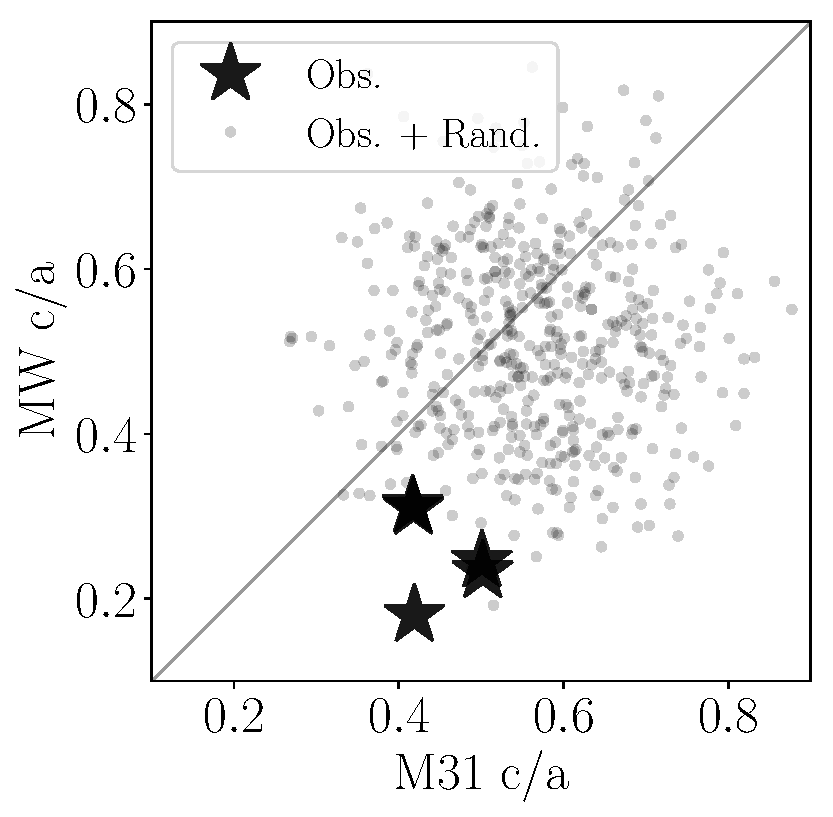
\includegraphics[width=0.30\textwidth]{scatter_random_ranked_ca_ratio.pdf}
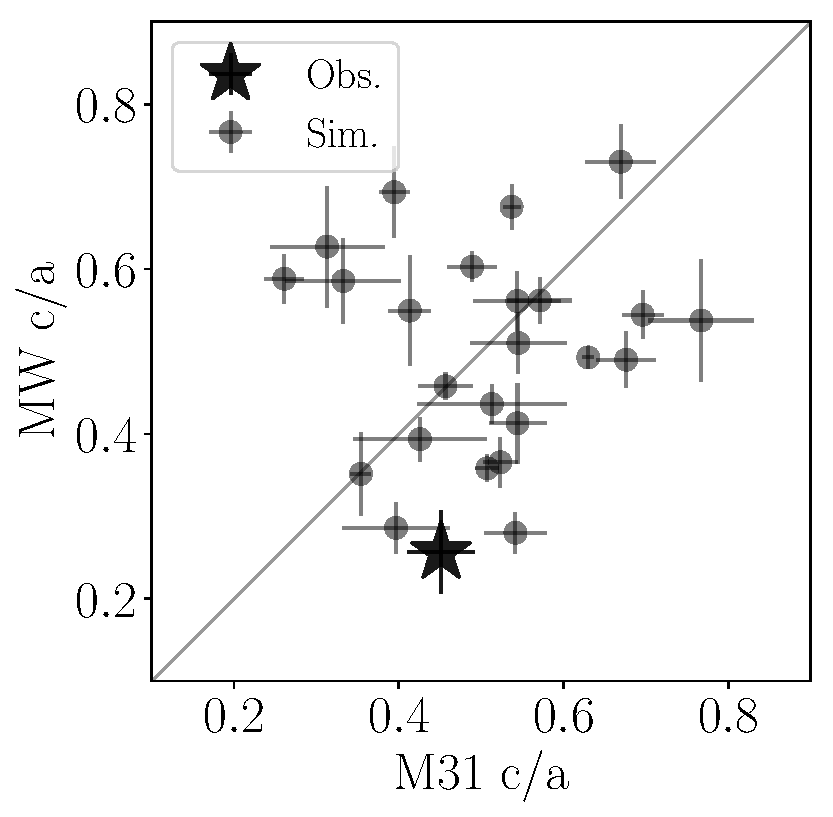
\includegraphics[width=0.30\textwidth]{scatter_ranked_illudm_ca_ratio.pdf}
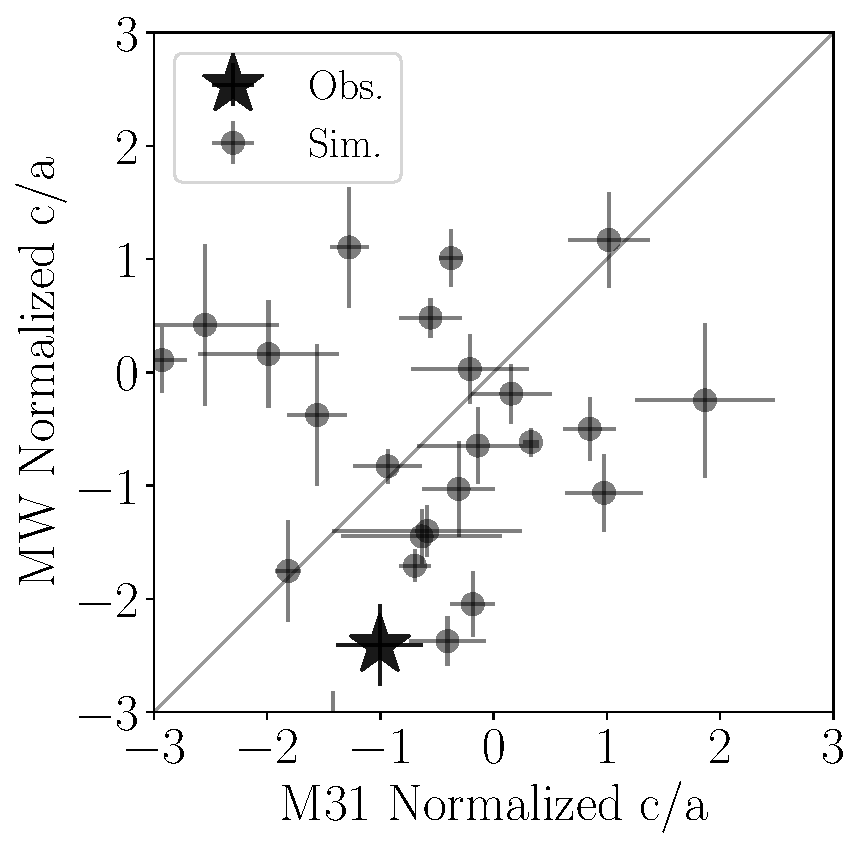
\includegraphics[width=0.30\textwidth]{scatter_norm_ranked_illudm_ca_ratio.pdf}
\caption{Same layout as in Figure \ref{fig:scatter_width}. 
This time for the $c/a$ axis ratio. 
The same message holds in this case; namely, that 
the MW has a significantly lower $c/a$ value than the
expectation from the spherical distribution and from the simulations. 
This low value is also $2\sigma$ away from the expactations for a
spherical distribution.
On the other hand, M31 is consistent both with a spherical
distribution and with the results from simulations.
\label{fig:scatter_ca_ratio}}
\end{figure*}


\begin{figure*}
\centering
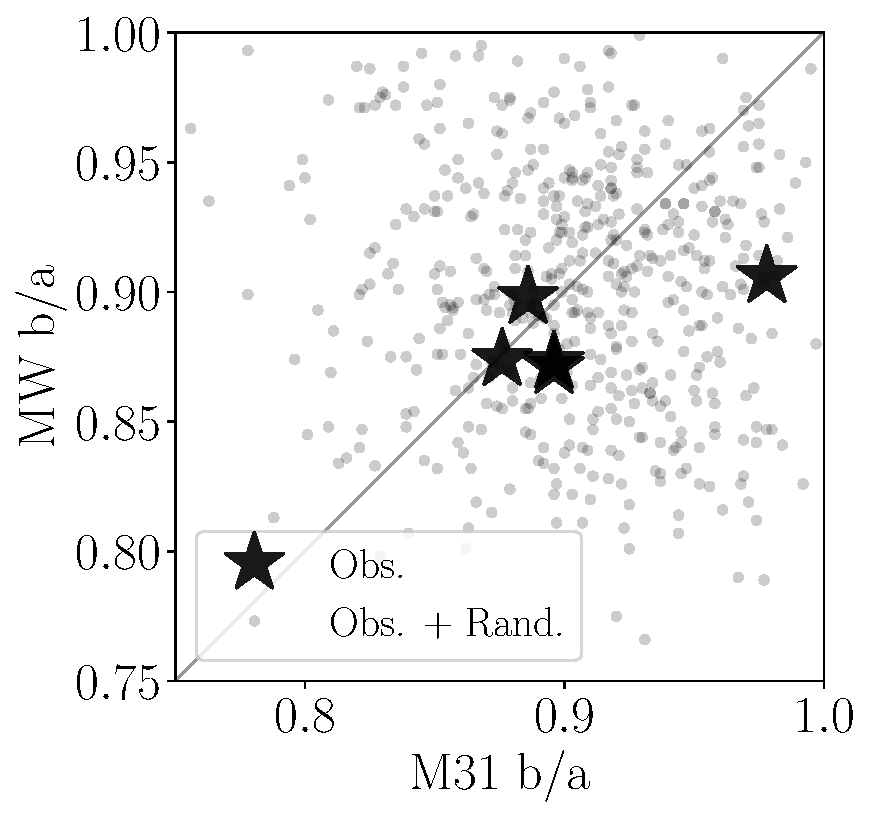
\includegraphics[width=0.30\textwidth]{scatter_random_ranked_ba_ratio.pdf}
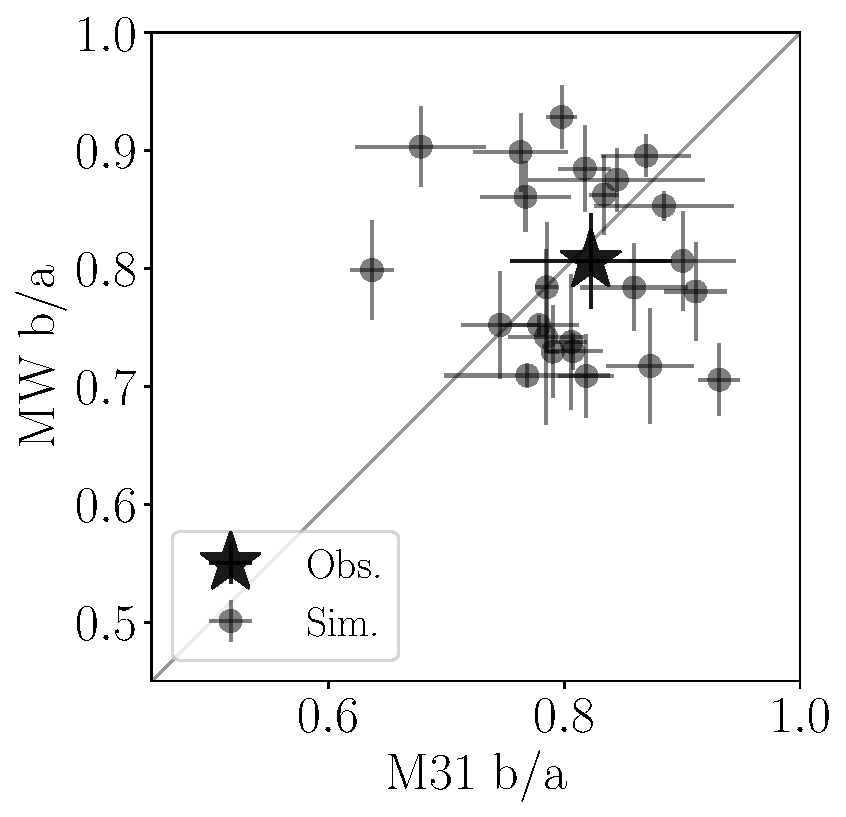
\includegraphics[width=0.30\textwidth]{scatter_ranked_illudm_ba_ratio.pdf}
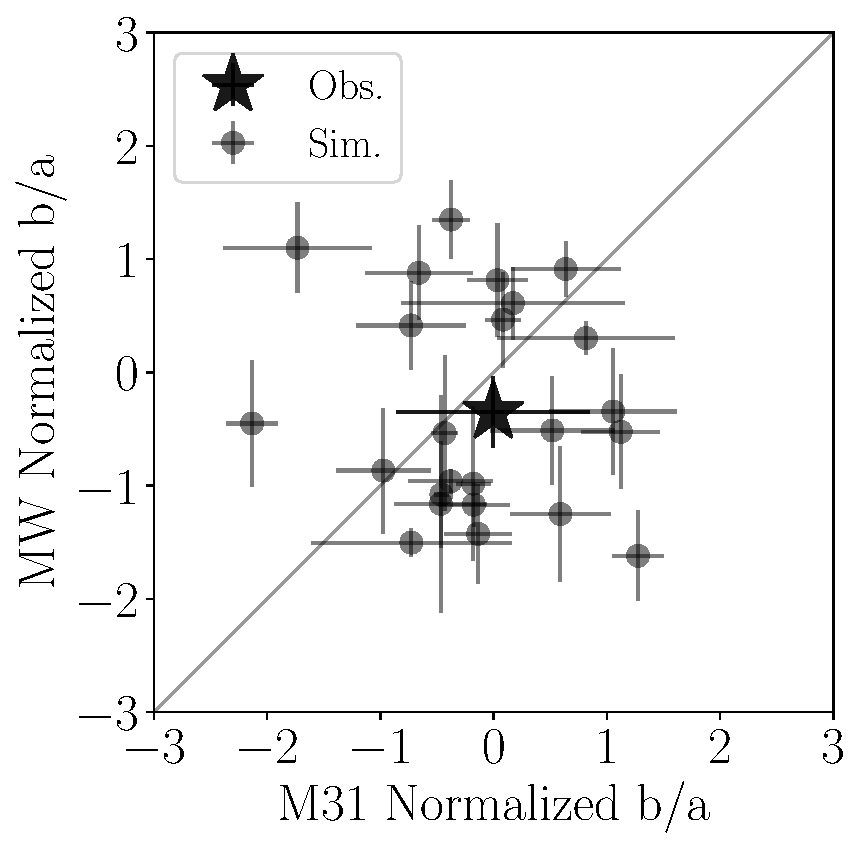
\includegraphics[width=0.30\textwidth]{scatter_norm_ranked_illudm_ba_ratio.pdf}
\caption{Same layout as in Figure \ref{fig:scatter_width}. 
This time for the $b/a$ axis ratio. In this case both the MW and M31
are consistent with the results of a spherical distribution and 
the simulations. 
\label{fig:scatter_ba_ratio}}
\end{figure*}


\begin{figure*}
\centering
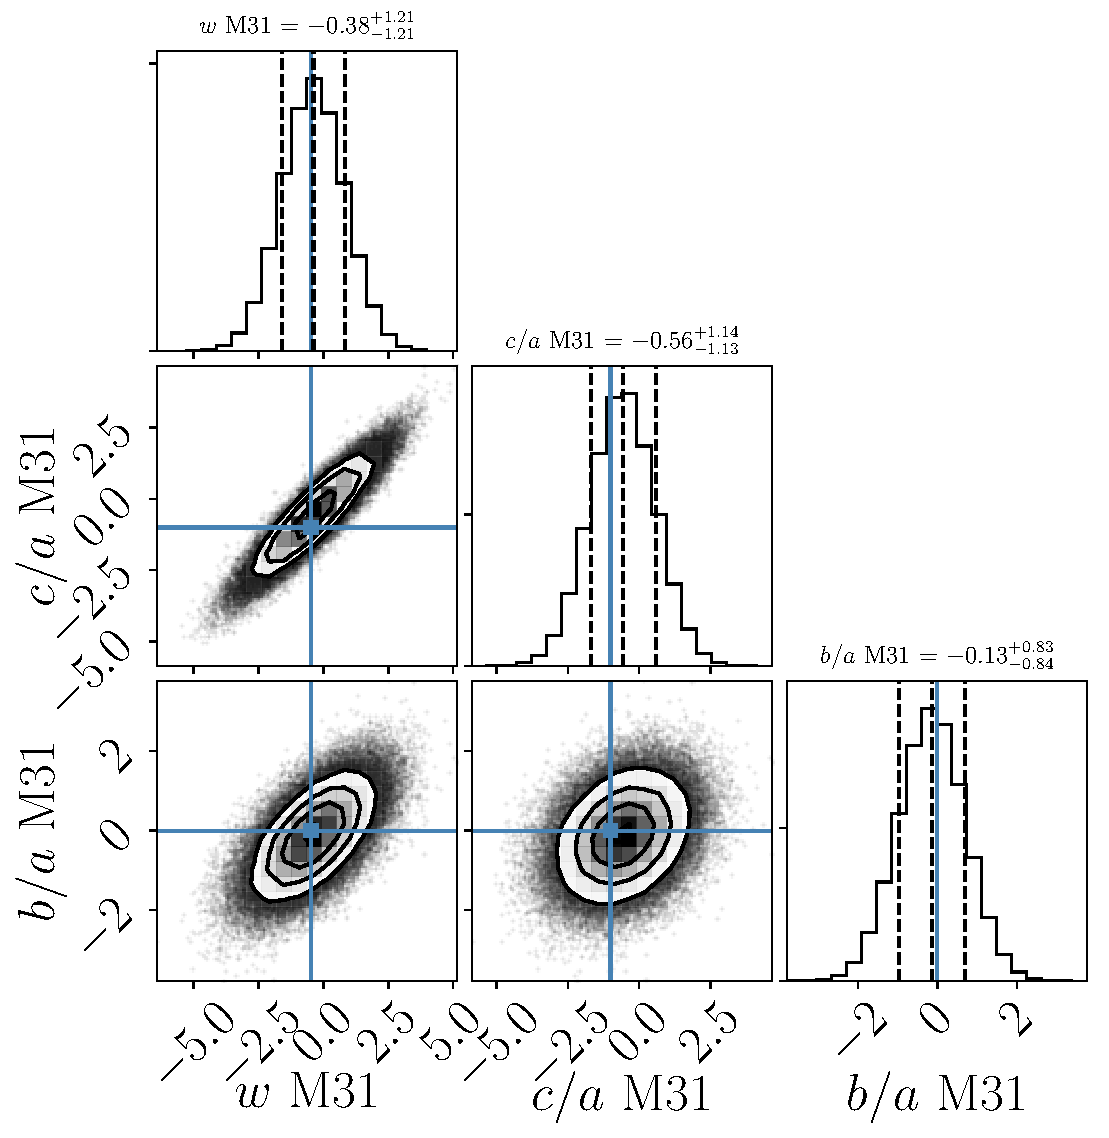
\includegraphics[width=0.45\textwidth]{gaussian_model_illustrisdm_M31.pdf}
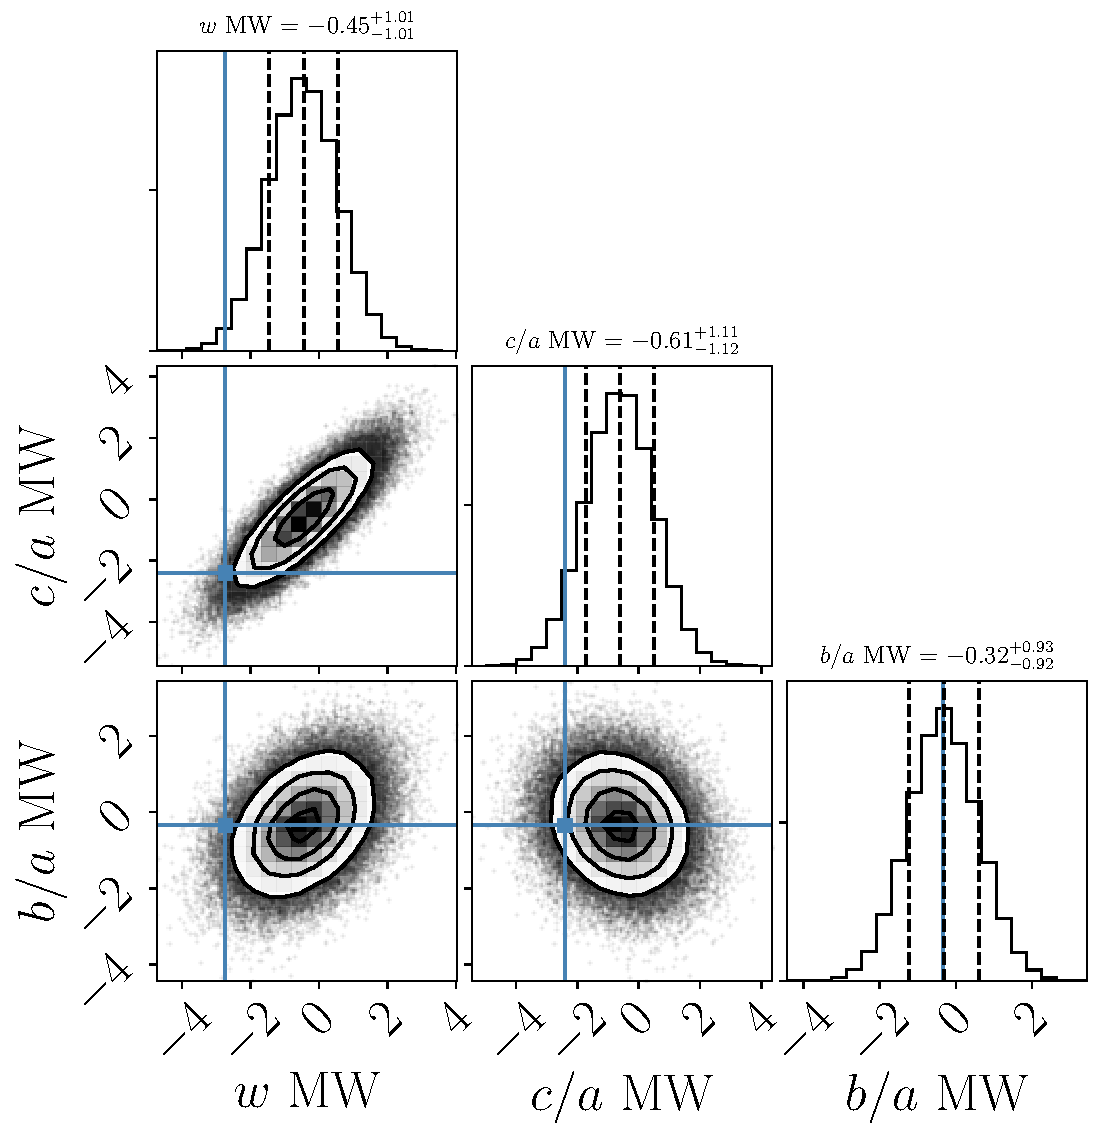
\includegraphics[width=0.45\textwidth]{gaussian_model_illustrisdm_MW.pdf}
\caption{Results from multivariate gaussian model fitted to the
  normalized values for the plane width $w$, $c/a$ ratio and $b/a$
  ratio from the Illustris1-Dark results.  
  Left/right panel correspond to M31/MW respectively.  
  The cross indicates the observed values.
  The contour levels in the 2D histograms correspond to the $1\sigma$,
$2\sigma$ and $3\sigma$ contours in two dimensions.
  The dashed vertical lines in the histograms along the diagonal
  correspond to the $1\sigma$ boundaries in one dimension.
  The results for the gaussian model are built from $10^6$ point
  realizations in the three-dimensional space spaned by the variables of
  interest for each halo. 
  This plot clearly shows how the M31 results are well within the
  expectations from simulations while the MW has an unusual low value for
  the plane width and the $c/a$ axis ratio.
\label{fig:correlations_illustrisdm}}
\end{figure*}


\section{Results}
\label{sec:results}

Table \ref{table:observations} and Table \ref{table:simulations}
summarize the mean values and uncertainties for the plane $w$, $c/a$
ratio and $b/a$ ratio in the observations and simulations, respectively. 
The uncertainty in the observations is computed from the results with
different number of satellites, while in the simulations it
corresponds to the standard deviation over different halos. 

The observed widths are always smaller than its randomized version.
For M31 there is barely a ratio of $0.92$ between observed and
randomized, while for the MW this factor goes down to less than half
$0.48$. 
The observed $c/a$ ratio follows the same extreme trend for
the MW compared to a M31 distribution closer to spherical, 
The $b/a$ ratio is statisically the same between observations and the
spherical randomization. 


In the following subsections we describe in detail the results on the 
distributions for $w$, $c/a$ and $b/a$. 
The plots in the main body of the paper correspond to the
Illustris1-Dark simulation; the results from the other simulations are
included in the Appendix.

\subsection{Plane Width}

Figure \ref{fig:scatter_width} summarizes the results for the width
measurements.
The left panel compares the results for the MW and M31
observations (stars) against its spherically randomized satellites
(circles). 
The most interesting outcome is that the MW plane width is smaller
than $\approx 98\%$ of the planes computed from the randomized distribution,
while the M31 plane width is only slightly smaller than the average of
the distribution.

The middle panel in Figure \ref{fig:scatter_width} compares the
observational result (star) against the measurements of all pairs from the Illustris1-Dark
simulation (circles).
In this case we have a similar result as before. 
The observed MW width is smaller than all the results in the
simulation, there is not a single halo with similar values.
On the other hand, the results for the M31 are entirely consistent
with observations. Most of the halos in the simulation show a width
value similar to M31. 

The right panel in Figure \ref{fig:scatter_width} shows the result for
the normalized width.  
This panel tells the same story as the middle panel. The M31 values
are typical while the MW is an outlier. 
The added value of the data in this panel is that it is the normalized
which is consistent with normal distributions.
This is the data used to build the mean values vector and covariance
matrix described in Equation \ref{} 



\begin{figure*}
\centering
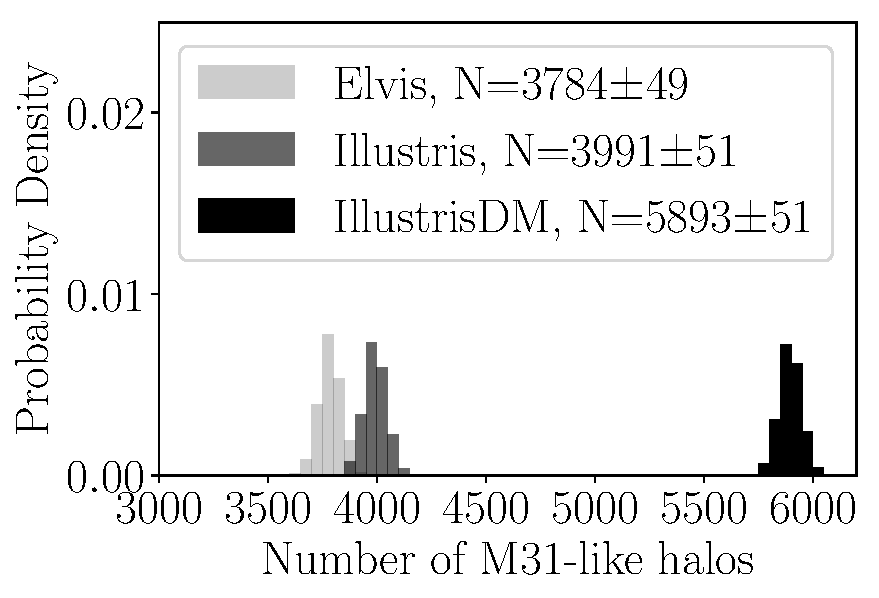
\includegraphics[width=0.47\textwidth]{expected_numbers_n_M31.pdf}
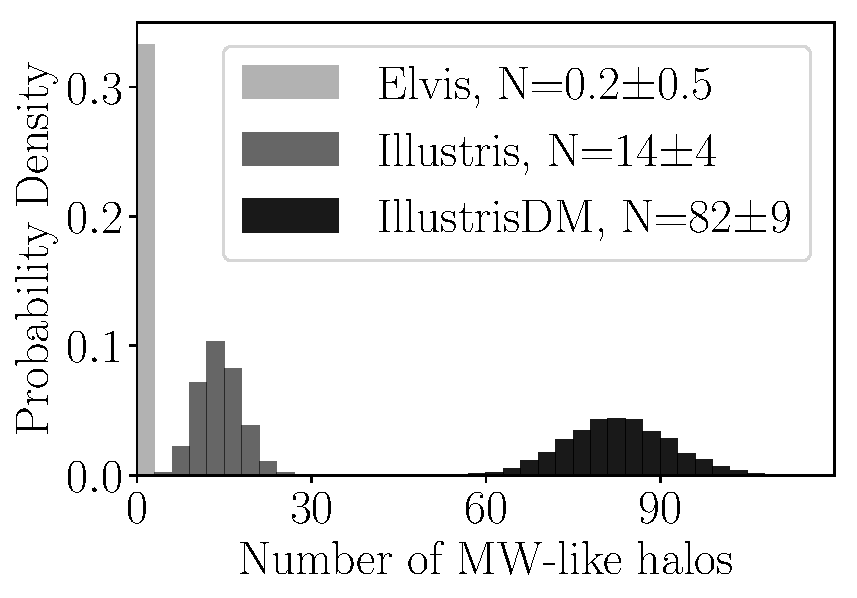
\includegraphics[width=0.47\textwidth]{expected_numbers_n_MW.pdf}
\caption{Probability distribution for the expected number of M31 and
  MW halos showing the same degree of atipicality as the Local Group if drawn
  from a sample of 10000 isolated pairs. 
  The distributions correspond to results derived from Illustris-DM, Illustris,
  and ELVIS data.
  In the most optimistic case (Illustris-DM), $1\%$ of the pairs have
  two halos with properties similar to the LG. In the case of
  Illustris this percentage drops to $0.1\%$ and $0.01\%$ for ELVIS.
\label{fig:expected_number}}
\end{figure*}

\subsection{$c/a$ axis ratio}

Figure \ref{fig:scatter_ca_ratio} shows the results for the minor to
major axis ratio. 
The layout is the same as in Figure \ref{fig:scatter_width}.
The results for the $c/a$ ratio follow the same trends as for the
width $w$.

The left panel in Figure \ref{fig:scatter_ca_ratio} shows how the MW
$c/a$ ratio is significantly lower than the measured values for
spherical distributions, and it is smaller than $\approx 98\%$ of the
randomized distributions.   
On the other hand the ratio for M31 is lower than the mean of the
spherical values but still well within its variance.
The middle panel in the same Figure shows the LG compared against the
results in the simulations. 
In this case we find a similar trend as before. 
The MW is atypical and M31 is within the variance from the simulation data.
This time, however, there are two MW-like halos out of the total
of 24 that show an $c/a$ as small as that of the MW.
The right panel shows the normalized results. 
The MW shows a low $c/a$ ratio close to between two and three
standard deviations away from the mean value of the spherical
distribution; this contrasts with the results for M31 which are close to
$1$ standard deviation away. 


\subsection{$b/a$ axis ratio}

Figure \ref{fig:scatter_ba_ratio} shows the results for the minor to
major axis ratio with the same layout as Figure \ref{fig_scatter_ca_ratio}
In all cases of comparison (against randomized distribution
and simulations) the results for both the MW and M31 are typical. 


\subsection{Fit to a Multivariate Gaussian Distributions}

Figure \ref{fig:correlations_illustrisdm} illustrates the results from
 computing the covariance matrix and mean vector in
 Eq.\ref{eq:multivariate} from the normalized quantities obtained from
 the Illlustris1-Dark simulation.
The distributions in this Figure are computed from $10^6$ with the multivariate
gaussian. 
Similar plots for Illustris1 and ELVIS are in the Appendix.
The values for all the covariance matrices and mean vectors
foricorresponding to all the simulations are listed in the Appendix.

This result nicely summarizes the results we had in the previous
sections. The left triangular plot shows how M31 falls into the middle of all 2D
distributions and is always close to the peak and within the $1-\sigma$
range. 
The right plot clearly places the MW observations outside the
$3\sigma$ range in the joint distributions that involve the width
$w$. 

In both cases the strongest positive correlation is present for the
width and the $c/a$ axis ratio. A weaker but still positive
correlation is present for the width and the $b/a$ axis ratio.



\subsection{Number of Expected LG Systems}

We use the fits to the multivariate gaussian distributions to
compute the expected number of pairs with characteristics similar to
those of the LG.
To do this we generate $10^3$ samples, each sample containing $10^4$
pairs, where each pair member is drawn from the corresponding
multivariate gaussian distribution.  

We consider that a sampled system is similar to the M31/MW galaxy if the
distance of each of its characteristics ($w$, $c/a$, $b/a$) to the
sample mean is equal or larger than the distance of the observational
values to the sample mean.   
That is, we perform a double-tailed test using the observational
values as a threshold. 

Figure \ref{fig:expected_number} summarizes the results from this
experiment. The left panel shows the probability density for the number of M31
systems in a parent sampe of $10^4$ pairs, the right panel shows the
results for the MW.
For M31, between $27\%$ and $56\%$ of the pairs have a satellite
distribution as aspherical as the observed in M31. This fraction drops
dramatically for the MW where only $0.02\%$ to $3\%$ of the satellites
are expected to have as extreme aspherical distributions as the MW.

Considering the joint distribution of M31 and MW we find that at most
$2\%$ of the pairs are expected to be similar to the LG.
In a three dimensional gaussian distribution, having a $1\sigma$,
$2\sigma$ and $3\sigma$ interval corresponds to have respectively $19 \%$, $73 \%$ and
$97 \%$ of the total of points in the distribution.
With this result in mind the $LG$ has the same degree of atipicality
as a $3\sigma$ outlier. 
% FUNDAMENTALS OF MULTIVARIATE STATISTICS, for Imaging and optics,
% Bajorski.
%In [150]: stats.chi2.cdf(l**2,3)
%Out[150]: array([ 0.19874804,  0.73853587,  0.97070911])

Among the three simulations, the results infered from ELVIS data show
the lowest fraction of M31 and MW systems; for Illustris1-Dark we have
the highest fraction of M31/MW systems. The results from Illustris1
are in between these two, but closer to ELVIS.

The most probable reason for these trends is the different median mass
for the MW/M31 halos in the pairs from these simulations. 
For instance for the MW halo the median maximum circular velocity is
$\sim 160$ \kms, $\sim 150$ \kms and $\sim 120$ \kms in the ELVIS,
Illustris1 and Illustris1-Dark simulations, respectively.
For the M31 halo this median velocity is $\sim 200$\kms both for the
ELVIS and Illustris1 simulations, while for the Illustris1-Dark it is
$\sim 160$ \kms. 


\section{Conclusions}\label{sec:conclusions}

In this paper we develop and demostrate a method to quantify the
asphericity of the satellite distribution in the around the MW and M31.  
In the interest of keeping the method straightforward and robust we do
not look for planes in subsets of satellites or coherent kinematical
structures. 
We focus on the asphericity estimates for a fixed number of the
brightest satellites around each galaxy.


The method uses as a reference the spherically randomized data
of the system under study \citep{2017AN....338..854P}.  
To this end, we first measure the width and axis ratios for the satellite
distributions of interest. 
Then, we measure the same quantities for the same set of points after
a process of spherical randomization.
Finally, we renormalize the initial results to the mean value and
standard deviation computed from the randomized data.  


We find that these normalized quantities are well described by
a multivariate gaussian distribution. 
We fit estimate the mean and covariance of this distributions using
the results of LG pairs coming from three different numerical
simulations, we inally compare the observational results against the
distributions derived from the simulations: Illustris-1,
Illustris-1-Dark and ELVIS.

We find that in the best case (Illustris1-DarkMatter) the deviation
from asphericity in the observed LG is only expected in $3\pm2$
pairs out of a sample of $10^4$ isolated pairs. This places the LG as
a $3\sigma$ outlier.   
The weight to explain this atypical result is not distributed equally
between the MW and M31. 
While M31 presents a fully typical asphericity in the expectations
from LCDM, the MW shows aspherical deviations in plane width and the
major-to-minor axis ratio highly atypical in the 
framework of LCDM. 
We estimate that with the M31 between $37\%$ and $58\%$ of the pairs
pairs show normalized characteristics larger than M31, while
this fraction drops to less than $1\%$ for the MW.
These fractions are robust to changes in the numerical simulations and to
the criteria used to define the pairs.


The highly aspherical distribution of the brightest MW satellites is
in stark contrast to the more spherical M31 distribution.
Furthermore, the atipicallity of the MW distribution in the LCDM
context adds up to the also atypical presence of two bright satellite
galaxies.


The focus of our approach is building explicit probability
distributions for the observables of interest, instead of trying to
find simulated objects that fulfill different observational criteria. 
This approach is particularly useful in the case of atypical
observables. 
Building the probability distribution allows for an atypicallity
quantification without needing to build explicit samples of objects
that are already scarce and difficult to find in simulations.

An extension of this framework to outliers in higher order deviations
(i.e. a \emph{subset} of satellites that are in a plane or
coherent \emph{velocity} structures) should also be possible, similar
to the work presented by XX\cite{2013Natur.493...62I} on the satellite velocity anisotropy.

From the results we derive in this paper we also estimate that a
cosmological volume of at least $( XX )^3$ is required to find a halo pair
that shows similar asphericity characteristics as the LG. 
This atypical satellite distribution should be seen as an opportunity
to constrain in high detail the initial conditions and environment
that allowed such a pattern to emerge. 


\section*{Acknowledgements} 
We acknowledge Universidad de los Andes and COLCIENCIAS (Project -
XXX) for the computing resources used in this project.


\bibliographystyle{mnras}
\bibliography{Dwarfs}

%% Alignments between galaxies, satellite systems and haloes
%% https://arxiv.org/pdf/1605.01728.pdf

%M31 mass
%% https://arxiv.org/abs/1410.0017

%MW mass
%https://arxiv.org/abs/1407.1078


\appendix

\section{Physical Characteristics of the Isolated Pairs samples}

\begin{figure}
\centering
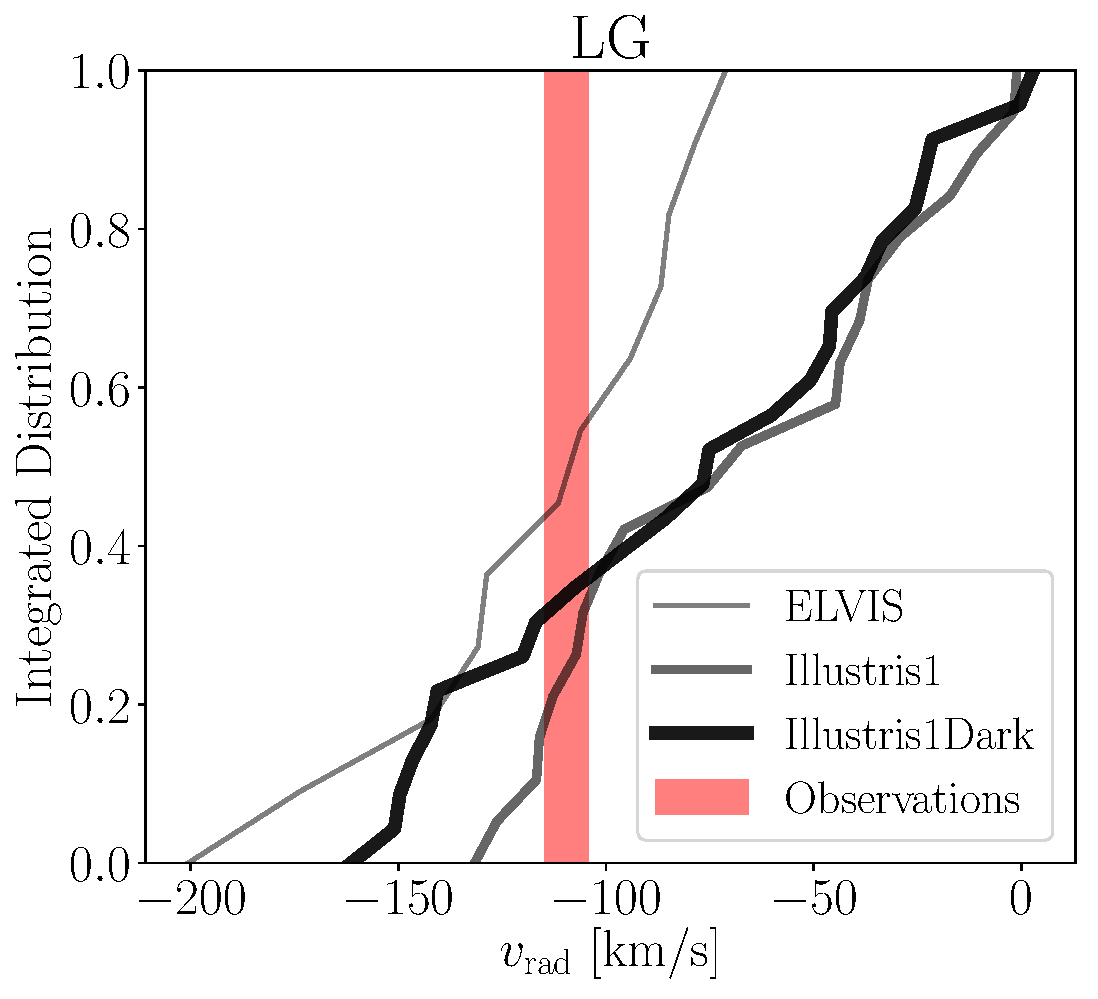
\includegraphics[width=0.34\textwidth]{int_distro_LG_v_rad.pdf}
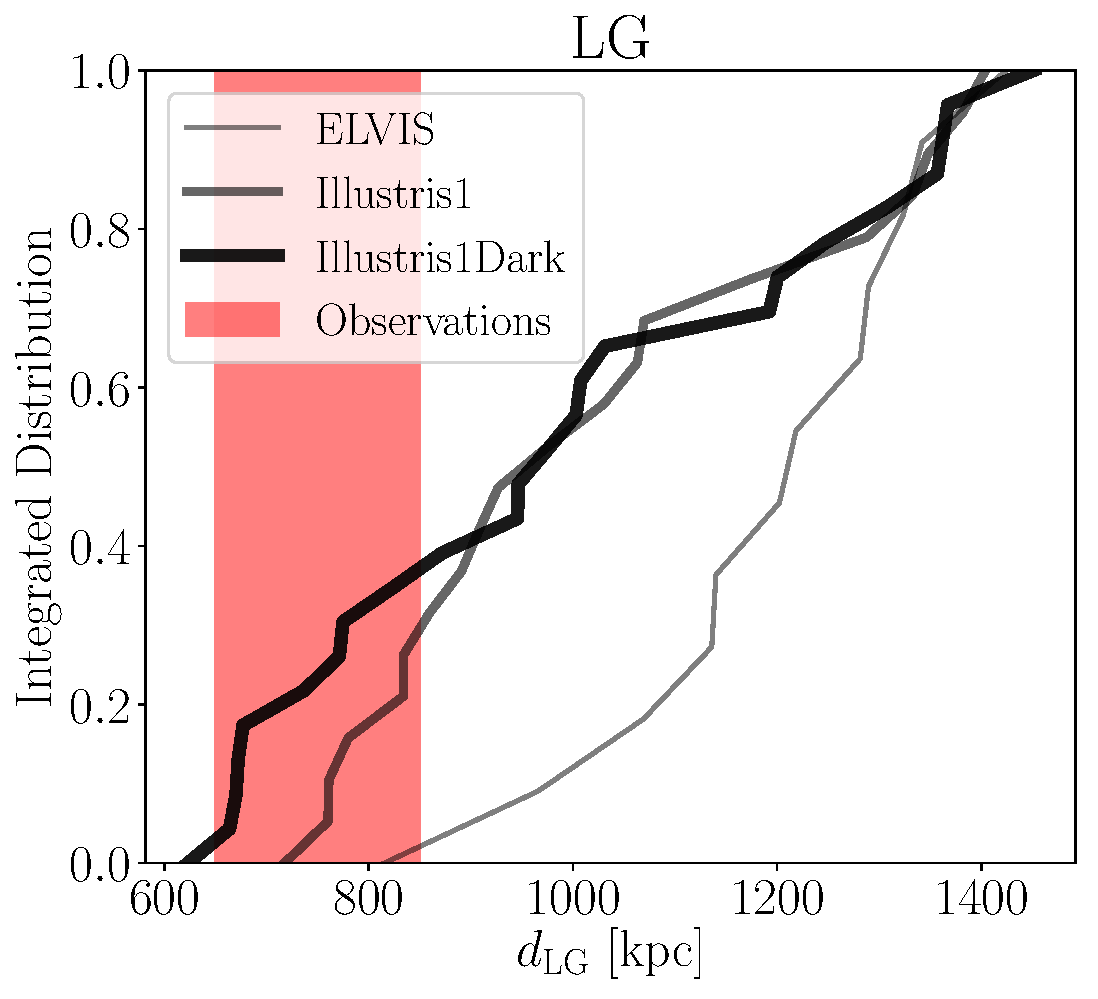
\includegraphics[width=0.34\textwidth]{int_distro_LG_d.pdf}
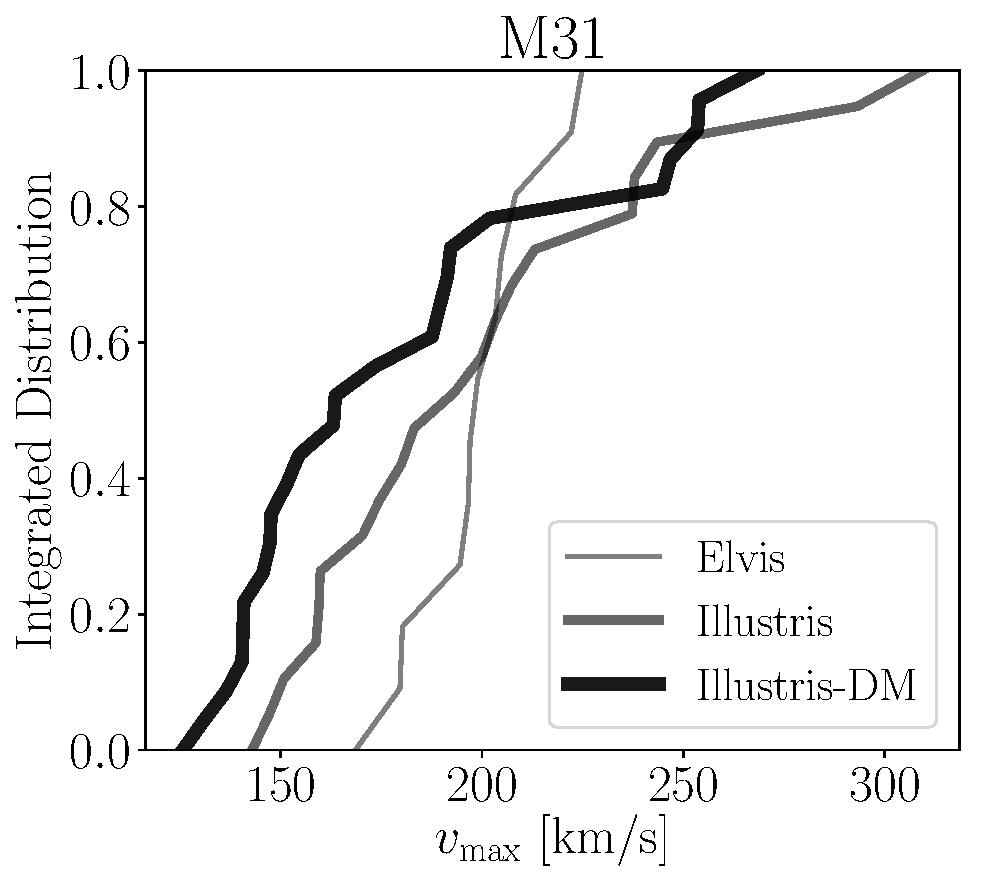
\includegraphics[width=0.34\textwidth]{int_distro_M31_vmax.pdf}
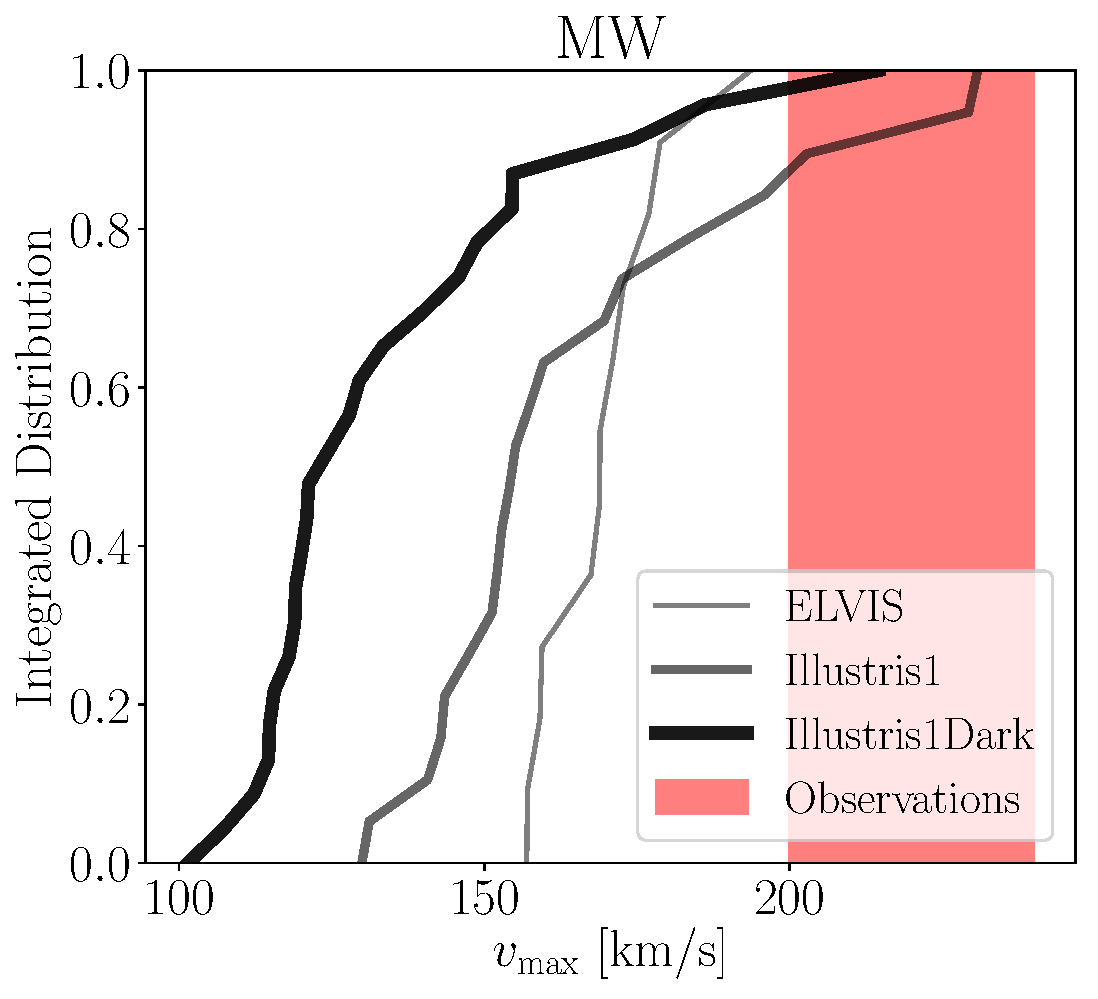
\includegraphics[width=0.34\textwidth]{int_distro_MW_vmax.pdf}
\caption{Physical characteristics of the LG pairs selected in the
  simulations. All lots show the integrated distributions. The
  physical properties are the radial comoving velocity between the MW
  and M31, the radial separation between the MW and M31 and the
  maximum circular velocity for the M31 and MW dark matter halo.
\label{fig:physical}}
\end{figure}

\section{Results from ELVIS and Illustris1}
\begin{figure*}
\centering
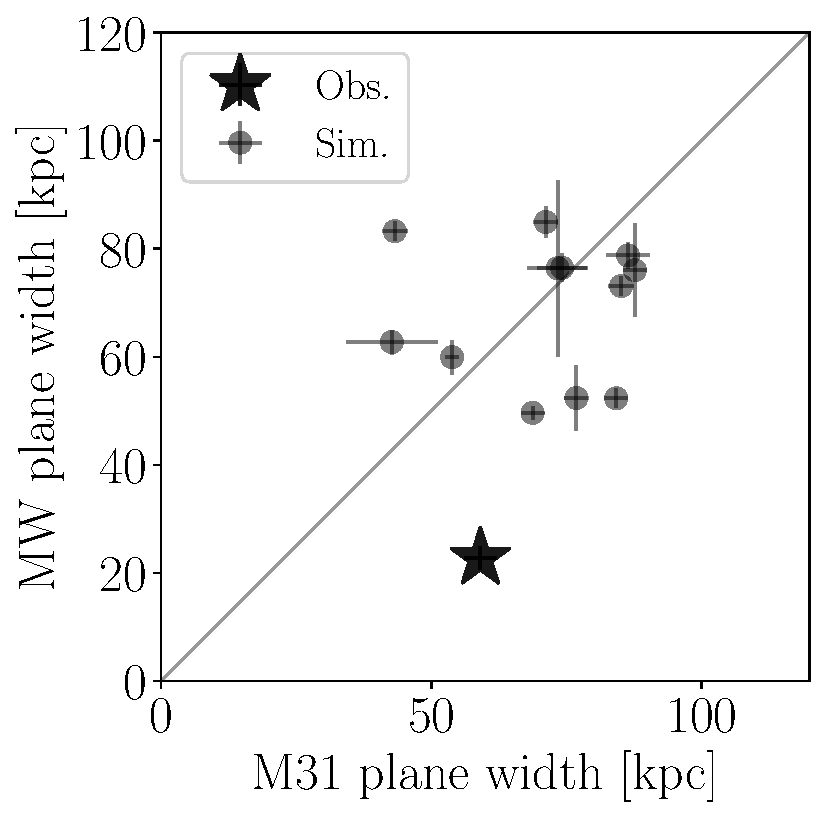
\includegraphics[width=0.32\textwidth]{scatter_ranked_elvis_width.pdf}
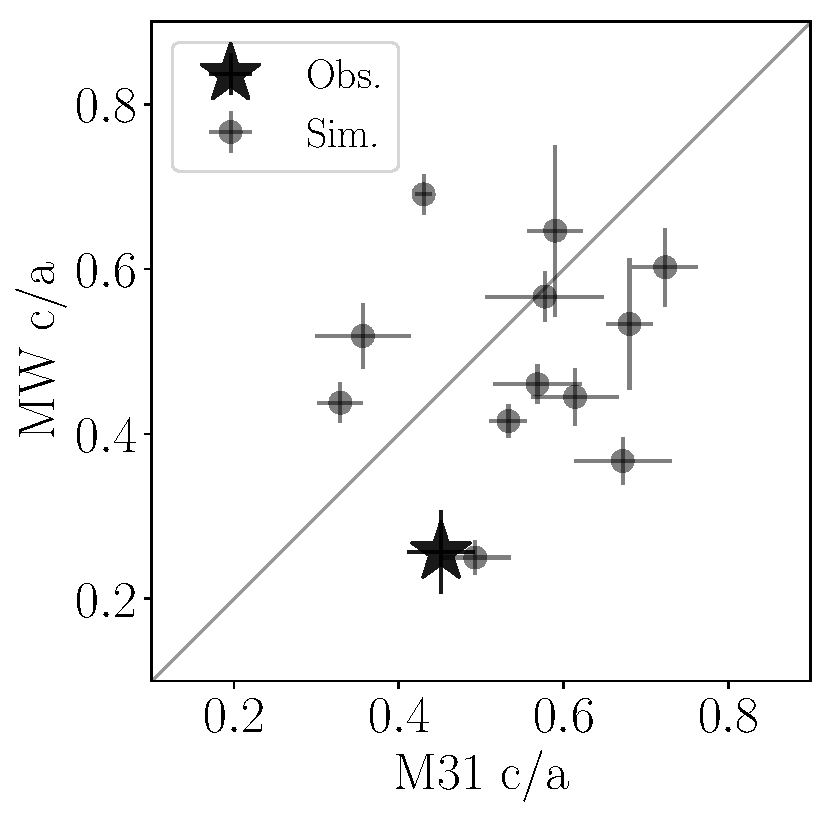
\includegraphics[width=0.32\textwidth]{scatter_ranked_elvis_ca_ratio.pdf}
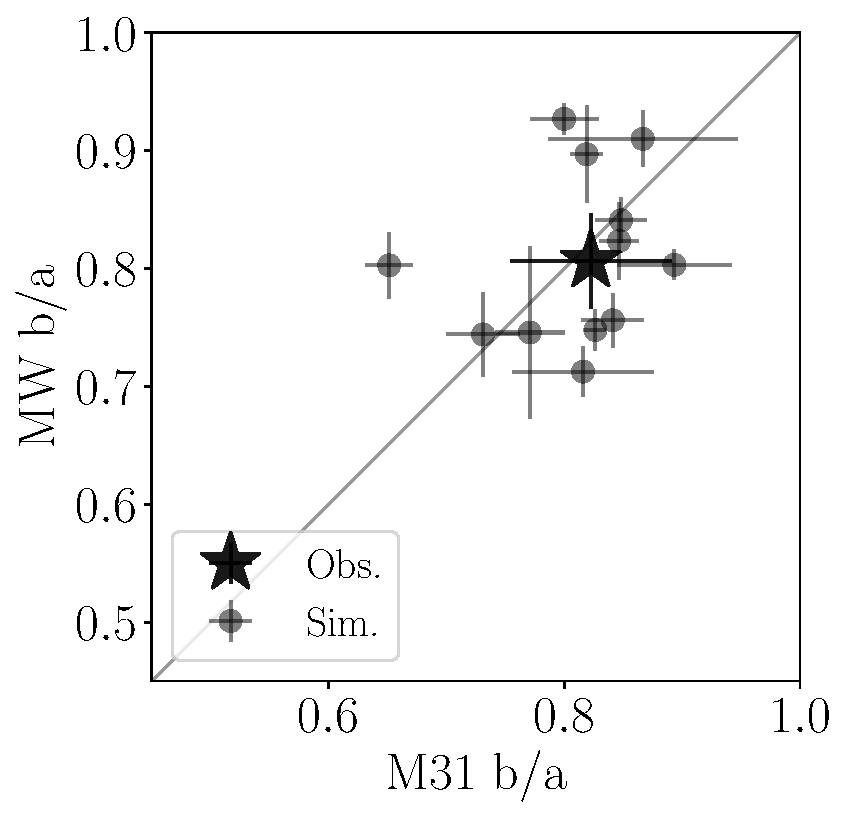
\includegraphics[width=0.32\textwidth]{scatter_ranked_elvis_ba_ratio.pdf}
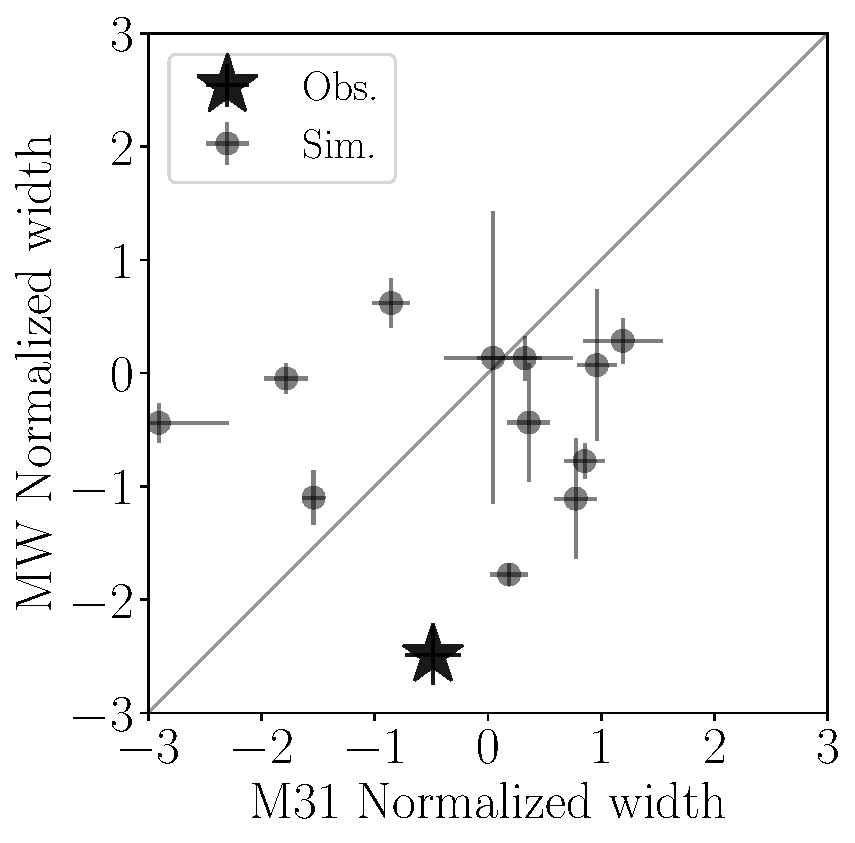
\includegraphics[width=0.32\textwidth]{scatter_norm_ranked_elvis_width.pdf}
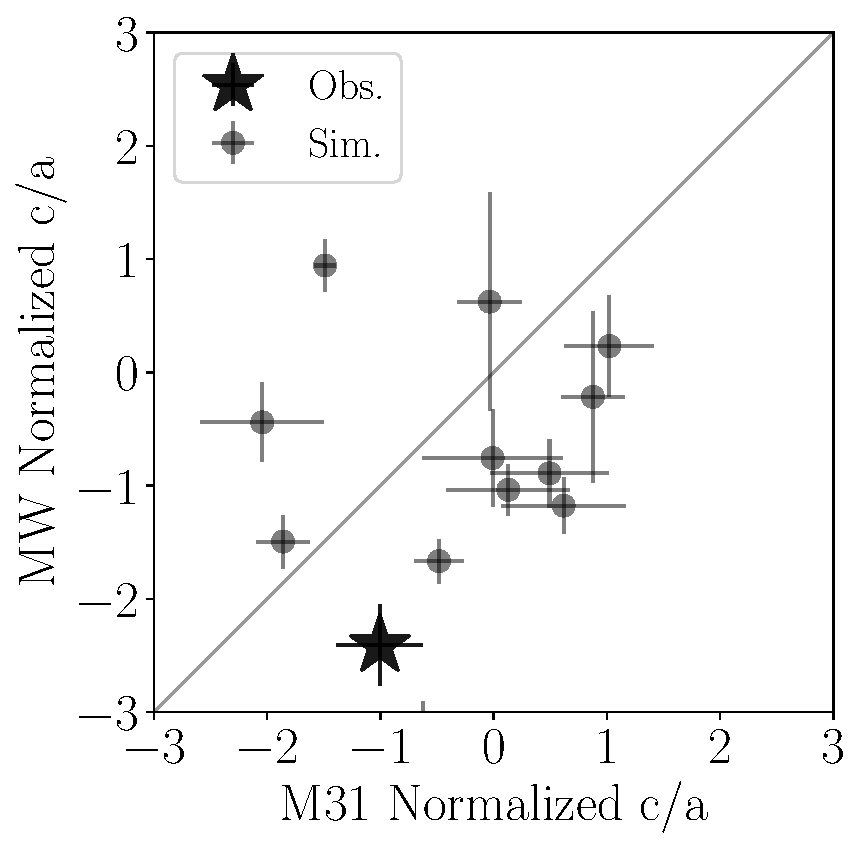
\includegraphics[width=0.32\textwidth]{scatter_norm_ranked_elvis_ca_ratio.pdf}
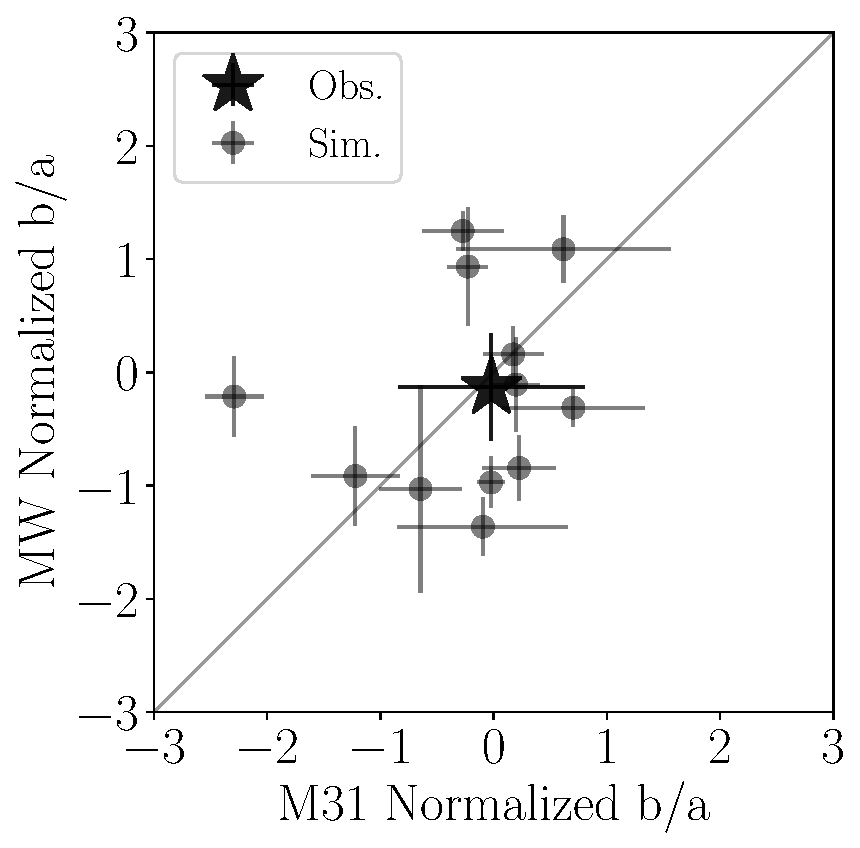
\includegraphics[width=0.32\textwidth]{scatter_norm_ranked_elvis_ba_ratio.pdf}
\caption{ELVIs results for the quantities presented for the Illustris1-Dark
  simulation in Figures  \ref{fig:scatter_width},
  \ref{fig:scatter_ca_ratio}, \ref{fig:scatter_ba_ratio}.
Upper row corresponds to the raw values from observations and
simulated pairs, while the second row normalizes the same values to
the mean and standard deviation on its spherically randomized
counterparts. 
\label{fig:scatter_elvis}}
\end{figure*}

\begin{figure*}
\centering
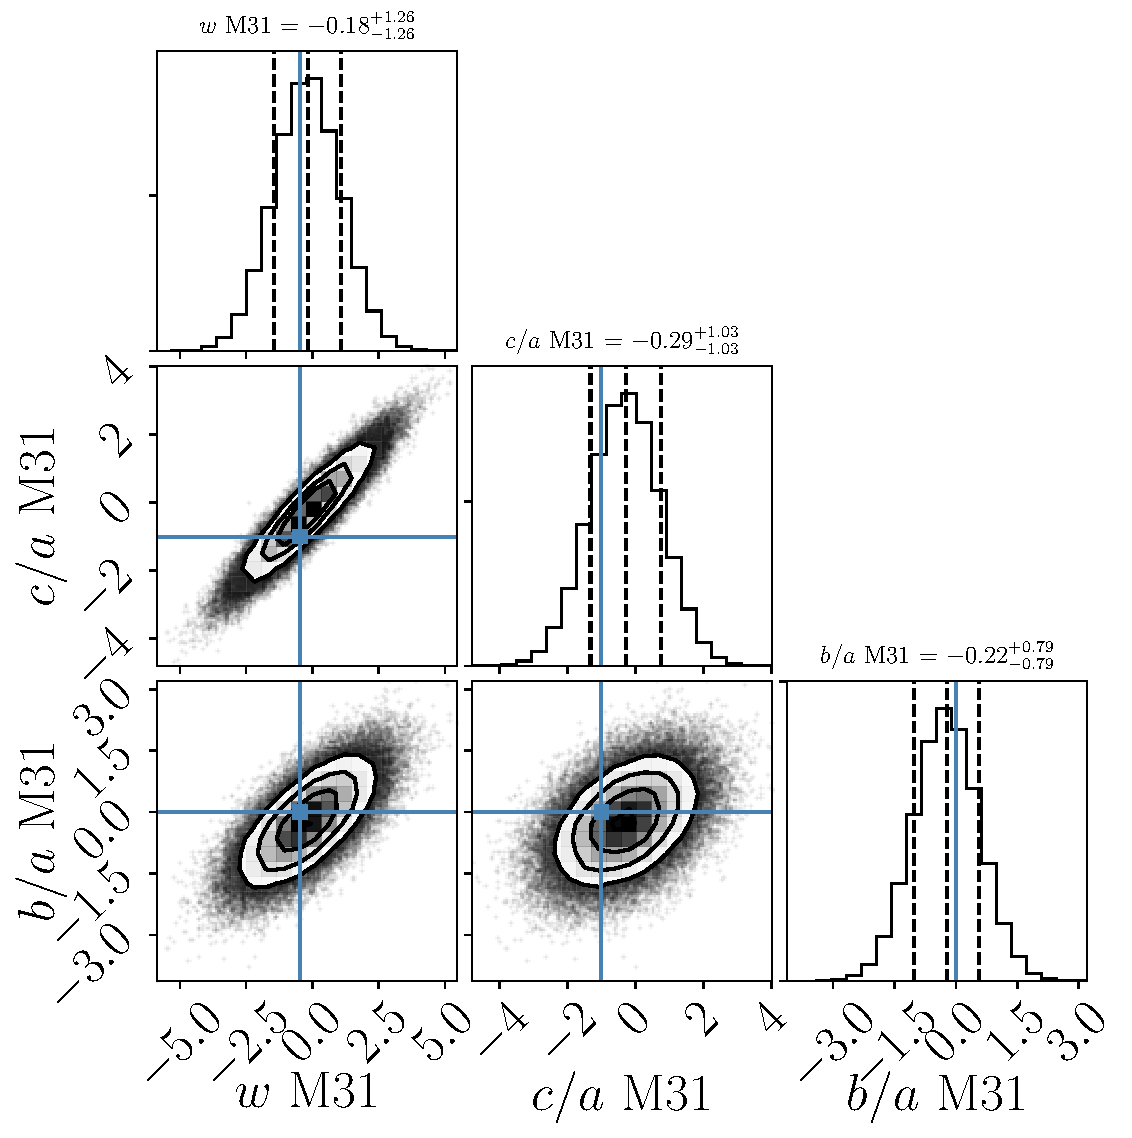
\includegraphics[width=0.48\textwidth]{gaussian_model_elvis_M31.pdf}
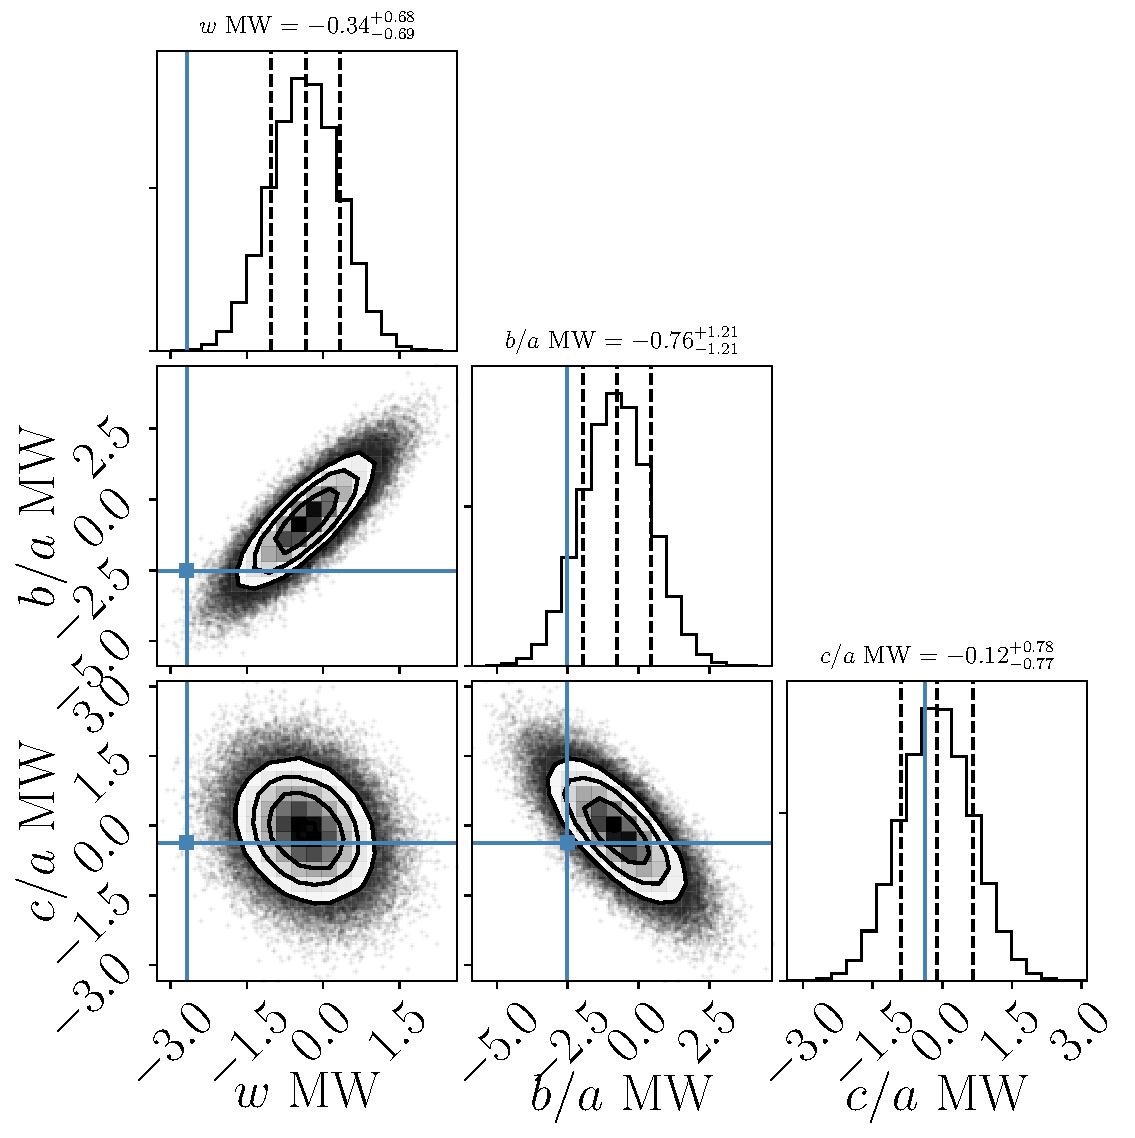
\includegraphics[width=0.48\textwidth]{gaussian_model_elvis_MW.pdf}
\caption{
Same layout as Figure \ref{fig:correlations_illustrisdm}, this time
computed from the ELVIS data.
\label{fig:correlations_elvis}}
\end{figure*}


\begin{figure*}
\centering
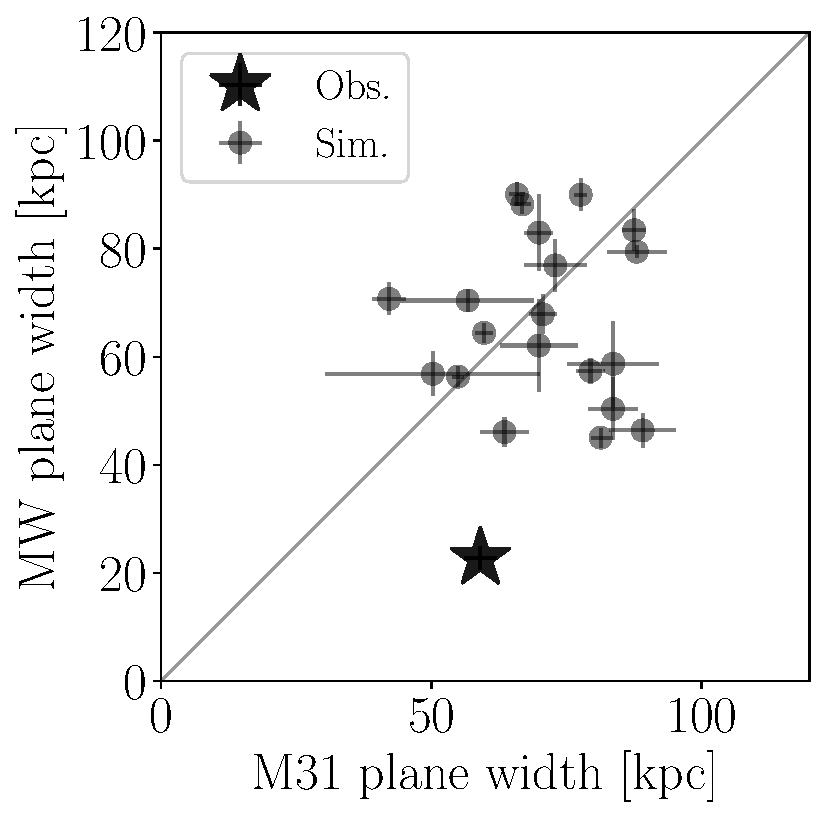
\includegraphics[width=0.32\textwidth]{scatter_ranked_width.pdf}
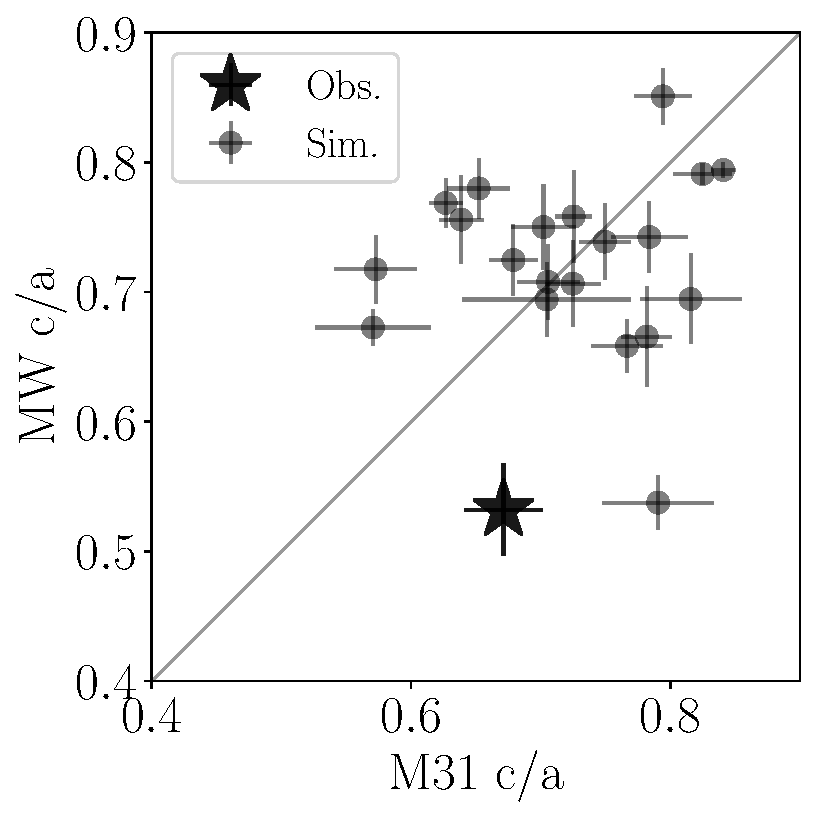
\includegraphics[width=0.32\textwidth]{scatter_ranked_ca_ratio.pdf}
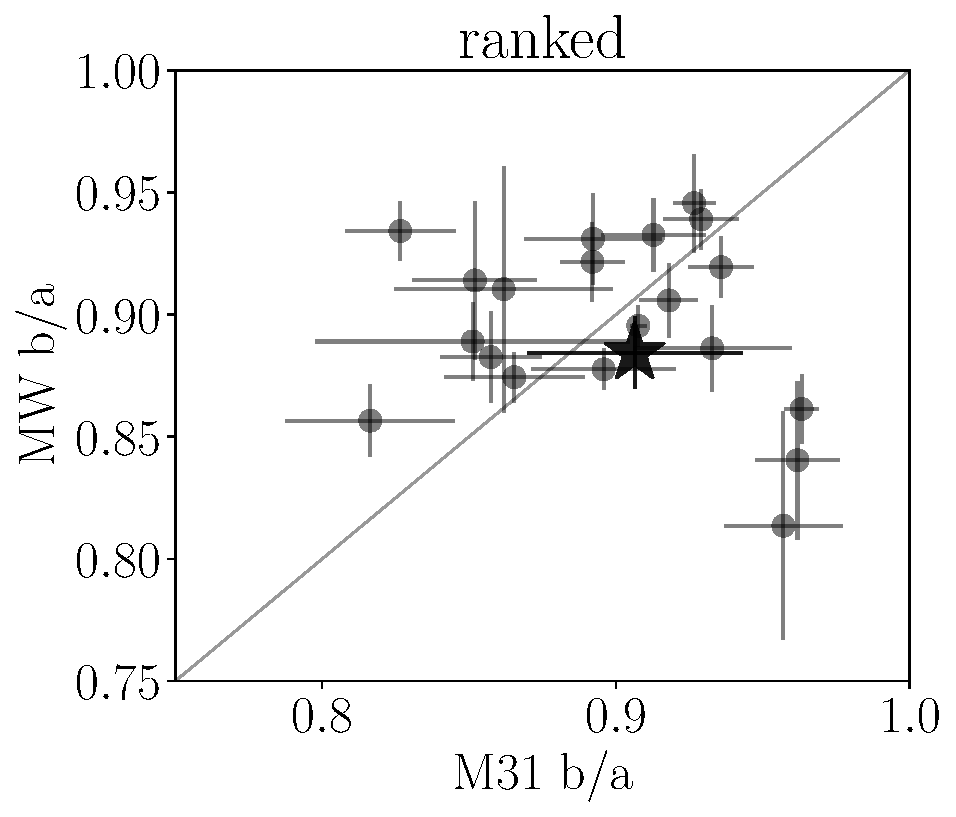
\includegraphics[width=0.32\textwidth]{scatter_ranked_ba_ratio.pdf}
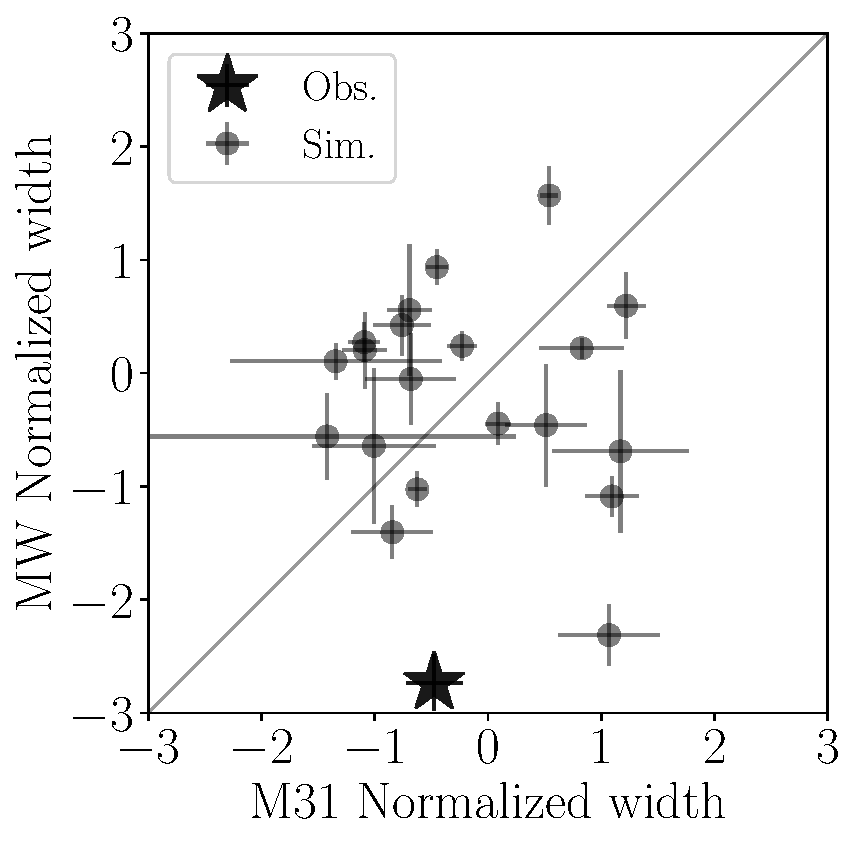
\includegraphics[width=0.32\textwidth]{scatter_norm_ranked_width.pdf}
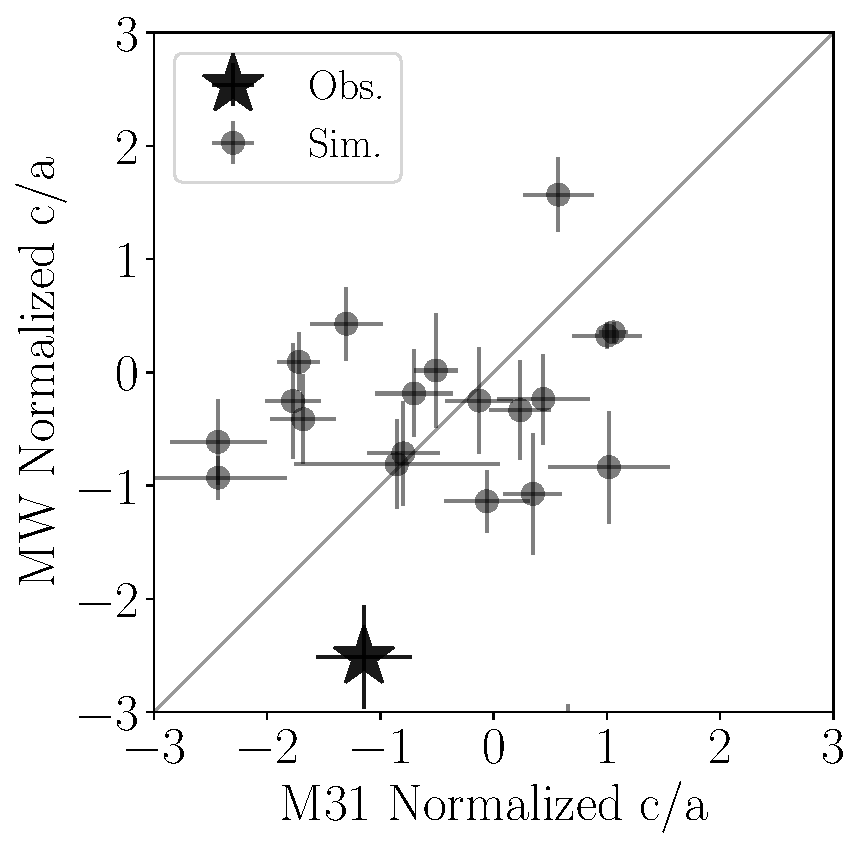
\includegraphics[width=0.32\textwidth]{scatter_norm_ranked_ca_ratio.pdf}
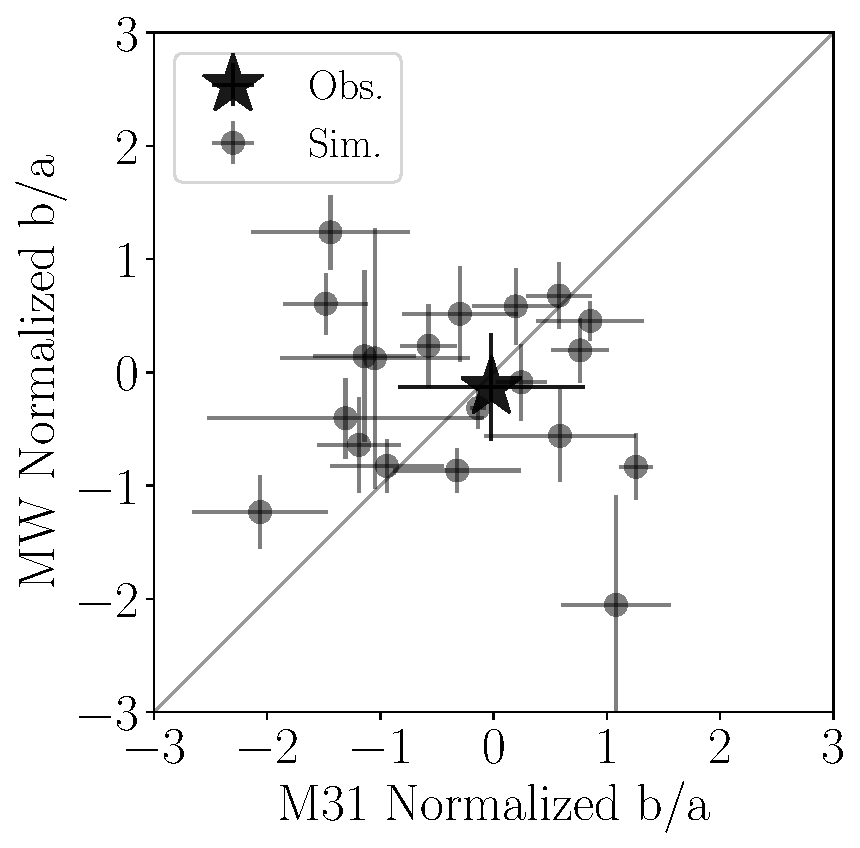
\includegraphics[width=0.32\textwidth]{scatter_norm_ranked_ba_ratio.pdf}
\caption{Same layout as Figure \ref{fig:scatter_elvis}, this time
  computed from the Illustris1 data.
\label{fig:scatter_illustris}}
\end{figure*}


\begin{figure*}
\centering
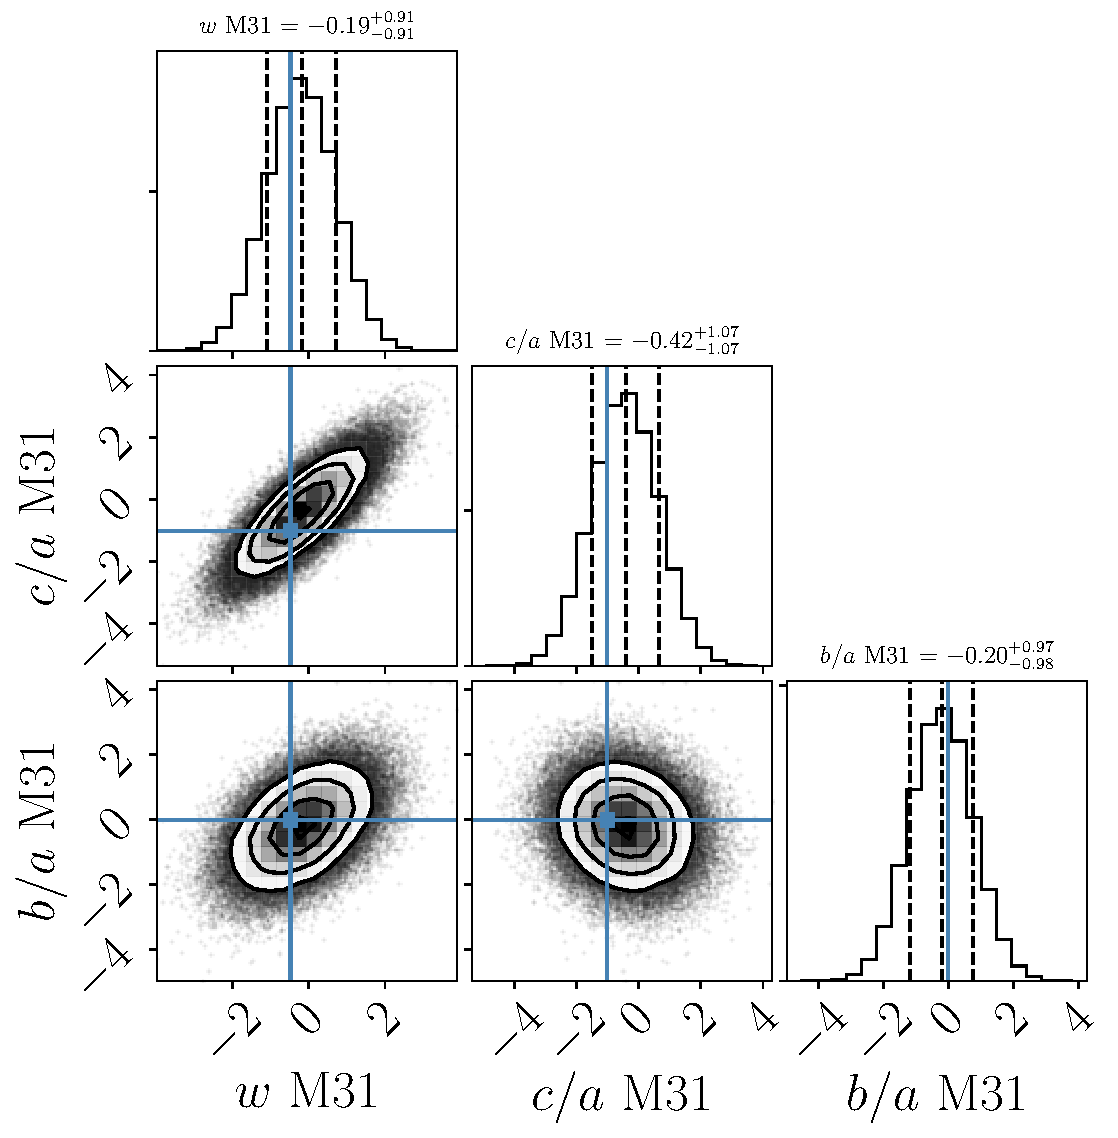
\includegraphics[width=0.48\textwidth]{gaussian_model_illustris_M31.pdf}
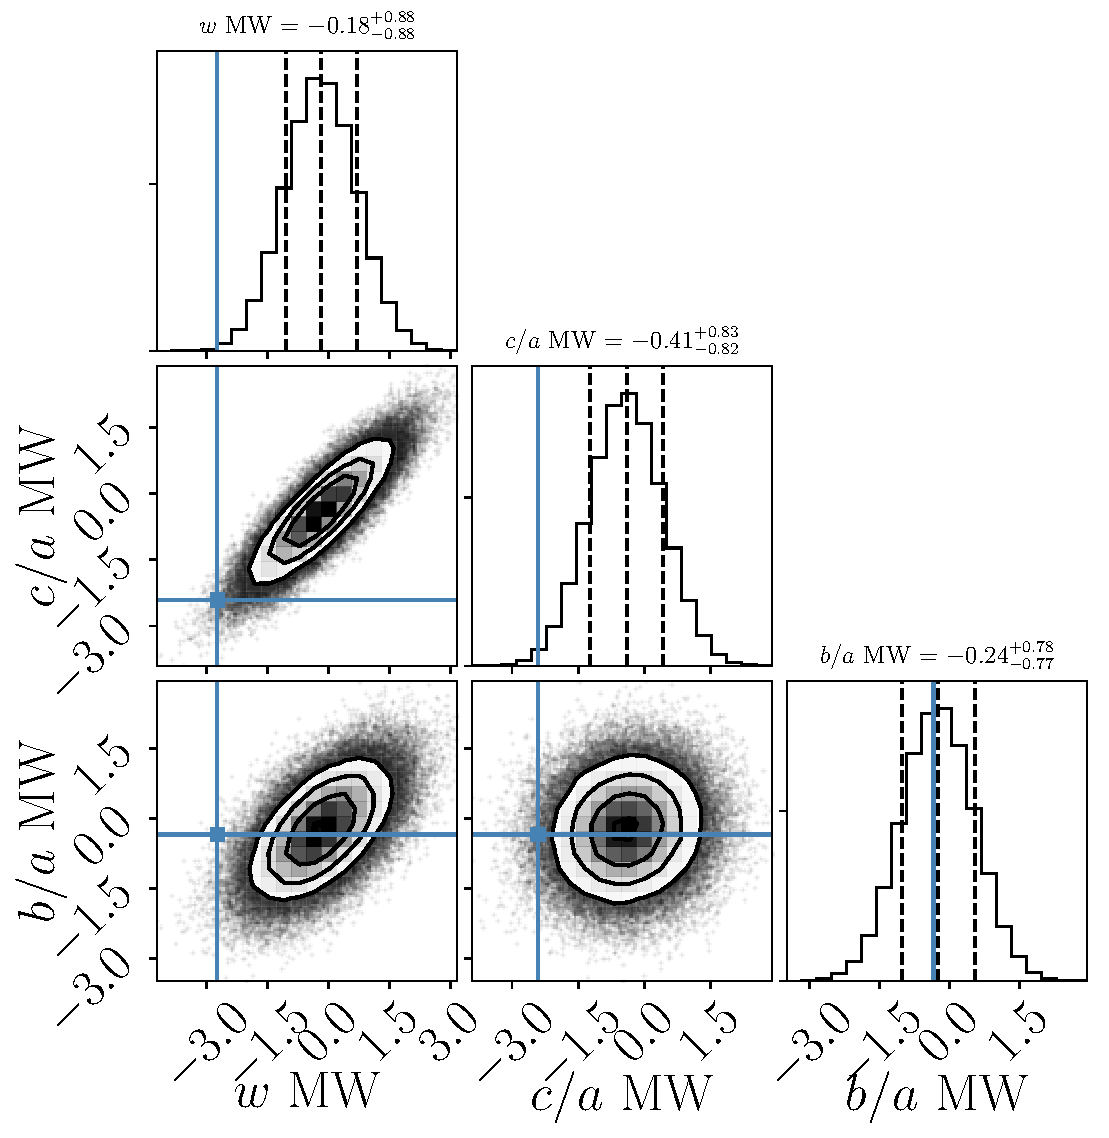
\includegraphics[width=0.48\textwidth]{gaussian_model_illustris_MW.pdf}
\caption{
Same layout as Figure \ref{fig:correlations_illustrisdm}, this time
computed from the Illustris1 data.
\label{fig:correlations_illustris}}
\end{figure*}


\newpage
\newpage
\section{Covariance Matrices and Mean value vectors}
\subsection{Illustris-1}

\subsubsection{M31}

\[
\Sigma= 
\begin{bmatrix}
0.83\pm 0.03  & 0.78\pm 0.04  & 0.41\pm 0.04\\
0.78\pm 0.04  & 1.16\pm 0.05 & -0.15\pm 0.05\\
0.41\pm 0.04 & -0.15\pm 0.05 & 0.96\pm 0.04\\
\end{bmatrix}
\]

\[
\mu= 
\begin{bmatrix}
-0.18\pm 0.04 & -0.41\pm 0.05 & -0.20\pm 0.05\\
\end{bmatrix}
\]

\subsubsection{MW}

\[
\Sigma= 
\begin{bmatrix}
 0.78\pm 0.06 & 0.63 \pm 0.07  & 0.40 \pm 0.03\\
  0.63\pm 0.07 & 0.69 \pm 0.08 &  0.06 \pm 0.02\\
  0.40\pm 0.03 & 0.06 \pm 0.02 &  0.61\pm 0.04\\
\end{bmatrix}
\]

\[
\mu= 
\begin{bmatrix}
-0.17\pm 0.04 & -0.40\pm 0.04 & -0.23\pm 0.04\\
\end{bmatrix}
\]

\subsection{Illustris-1-Dark}

\subsubsection{M31}

\[
\Sigma= 
\begin{bmatrix}
 1.50\pm 0.08 & 1.27\pm 0.08 & 0.64\pm 0.04\\
  1.27\pm 0.08 &  1.31\pm 0.08&  0.28\pm 0.04\\
  0.64\pm 0.04 &  0.28\pm 0.04 & 0.70\pm 0.04\\
\end{bmatrix}
\]

\[
\mu= 
\begin{bmatrix}
-0.37\pm 0.05& -0.55\pm 0.05 & -0.13\pm 0.03\\
\end{bmatrix}
\]

\subsubsection{MW}

\[
\Sigma= 
\begin{bmatrix}
 1.03\pm 0.05 & 0.94\pm 0.05  & 0.36\pm 0.03\\
  0.94\pm 0.05 & 1.24\pm 0.07 & -0.18\pm 0.04\\
  0.36\pm 0.03 & -0.18\pm 0.04  & 0.86\pm 0.03\\
\end{bmatrix}
\]

\[
\mu= 
\begin{bmatrix}
-0.45\pm 0.04 & -0.61\pm 0.05 & -0.31\pm 0.04\\
\end{bmatrix}
\]

\subsection{ELVIS}

\subsubsection{M31}

\[
\Sigma= 
\begin{bmatrix}
 1.60\pm 0.19  & 1.22\pm 0.14 & 0.70 \pm 0.09\\
  1.22\pm 0.14 &  1.08\pm 0.10 & 0.35 \pm 0.05\\
  0.70\pm 0.09 & 0.35\pm 0.05  & 0.63 \pm 0.10\\
\end{bmatrix}
\]

\[
\mu= 
\begin{bmatrix}
-0.18\pm 0.08 & -0.28\pm 0.07 &-0.22\pm 0.05\\
\end{bmatrix}
\]

\subsubsection{MW}

\[
\Sigma= 
\begin{bmatrix}
 0.45\pm 0.04 & 0.61\pm0.09 & -0.11\pm0.09 \\
  0.61\pm0.09 & 1.21\pm0.17 & -0.63\pm0.09\\
 -0.11\pm0.05 & -0.63\pm0.09 & 0.64\pm0.06\\
\end{bmatrix}
\]


\[
\mu= 
\begin{bmatrix}
-0.32\pm 0.04 & -0.74\pm 0.07 &-0.08\pm 0.05\\
\end{bmatrix}
\]


\end{document}
